\documentclass[12pt]{article}
\title{Advanced Machine Learning: Final Project} 
\author{
	Aman Gulati \\
	ag3743 \\
	\and 
	Joaquim Lyrio  \\
	jc4637 \\
	\and 
	Ricardo Pommer \\
	rap2194 \\
	\and
	Henrique Saboya \\
	hs2923 \\
}

\usepackage{bbm, pifont, amsmath, enumerate, amssymb, pdfpages, graphicx, caption, float}

\newcommand{\reals}{I\!\!R} %real numbers
\captionsetup[figure]{font = small, labelfont = bf}

\begin{document}
\maketitle

\begin{abstract}
	Neural networks, although empirically validated, remain a theoretically opaque tool. Once we have trained a particular architecture, what within its layers, neurons, or channels, drive its classification performance? How do we interpret the results beyond out-of-sample loss measures? Feature visualization attempts to elucidate this question by, generally speaking, projecting intermediate layers to pixel-space. In this report,  we review and consolidate different methods of feature visualization, their definitions, theoretical approaches and results on three neural network architectures and datasets.
\end{abstract}

\subsection{Definitions}
As any young field, neural networks and their interpretability has yet to agree on definitions for a vast number of methods and parameters. Feature visualization often produces compelling images, but their contribution to the interpretation of a neural network depends on clear definitions of each procedure. Here, we provide our own. Although they may at times conflict with other authors', we hope these will contribute to the specificity of our discussion.

\subsubsection{Feature Visualization:}
We refer to \textbf{feature visualization} as any projection onto pixel-space that relays information about a (generally hidden) subset of the network's architecture. This is a particular approach to the general problem of \textbf{neural network interpretability}. Some authors (Olah et al., 2017) \cite{distill} distinguish between \textbf{feature visualization} and \textbf{attribution}, defining the former as the generation of maximum activation images through optimization, while the latter looks for specific inputs that generate layer (or node)-specific activation. We draw no such distinction.

\subsubsection{Features:}
Subsets of any data set, either in the input or hidden within the network. Generally, however, we prefer to use features to characterize the input data.

\subsubsection{Feature Map:}
The output of a single kernel applied to data flowing through a network. This can be used interchangeably with \textbf{activations}.

\subsubsection{Weight Visualization:}
The simplest and canonical form of feature visualization: plotting \textit{trained} weights of a hidden node (term which we use interchangeably with \textbf{filter}) or layer directly, regardless of dimension.

\subsubsection{Feature Map Visualization:}
The next-simplest approach is to pass a given image through a \textit{trained} node or layer and visualize directly. This is, from our above definition, \textbf{feature maps} visualization of intermediate layers. Again, we make no restriction on the dimensionality, since we expect feature maps to have different dimensions depending on its position in the layer's architecture.\\

A useful analogy with the physical world is quite immediate: we shine our input image through a trained filter, and see what comes out on the other side. Since we know what our original image looks like, seeing the difference between input-output should give us some insight about the filter. Contrastingly, \textbf{weight visualization} looks at the ``filter" directly, while \textbf{feature map visualization} looks at the image \textit{through} the ``filter" (using filter loosely and in reference to a physical filter and not necessarily a node in a convolutional layer). Much of this procedure is based on the package \textbf{``tf\_cnnvis"} \cite{cnnvis}.

\subsubsection{Deconvolutional Projection:}
Unlike feature-map  visualization, \textbf{deconvolutional projection} attaches something similar to an auto-encoder network, or \textbf{deconvolutional network} after each node. The methodology followed is almost identical to (Zeiler \& Fergus, 2013) \cite{zeiler}, with the exception that due to computational constraints we do not save max-pool locations and instead pass the maximum to the entire relevant area \cite{oxford, kvfrans}. \\

Technically, the output of a deconvolutional network is still a feature-map but we avoid using the term to avoid confusion, particularly when discussing their visualization.

\section{A Simple (But Useful) Example}
To motivate our survey, we begin with a toy model and dataset of the letters ``E", ``F" and ``L". The network and dataset are based on (Orbanz, 2017) as presented in lecture notes and a sample is shown in \textit{Figure 2}. We generate 2,000 images of each category and add noise distributed as $\mathcal{N} \sim (0, 0.2)$, with all negative noise samples regularized to 0. Following, we train a 1-hidden layer neural network classifier, as shown in \textit{Figure 1}. \\

\begin{figure}[h]
\centering
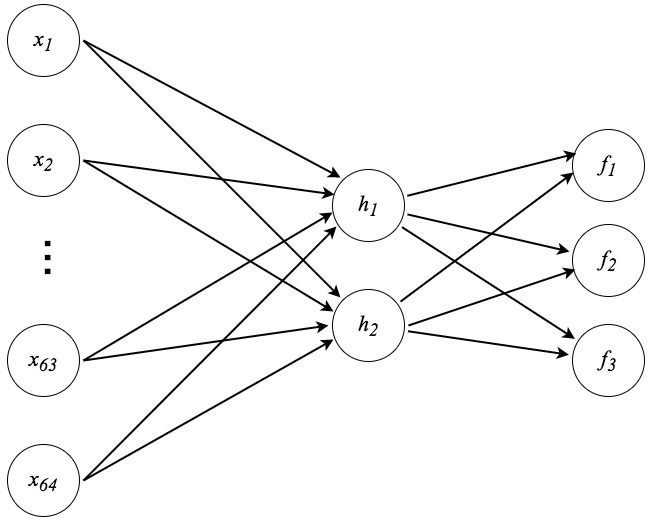
\includegraphics[width=0.7\linewidth]{../diagrams/EFL_network}
\caption{Training set: 3,333 per category. Test set: 400 per category.\\ Train error: ~0 \%. Test error: ~0\%. Training time (black letters): 14 seconds. Training time (white letters): 21 seconds.}
\label{fig:eflnetwork}
\end{figure}

\begin{figure}[h]
	\centering
	\includegraphics[width=0.7\linewidth]{../../../../../../../Desktop/efl_sample}
	\caption{Sample from EFL datset}
	\label{fig:eflsample}
\end{figure}

\pagebreak

Note that we do not include biases or convolutions-- the nodes are simply matrix multiplying the weights by the input image, before passing through a reLu non-linearity. This simple structure allows us to visualize the weights directly. \\

\begin{figure}[h]
\centering
\includegraphics[width=0.7\linewidth]{../../../../../../../Desktop/efl_1}
\caption{Trained weights of nodes $h_1$ and $h_1$. White pixels are close to 1, and black pixels are closest to 0. Clear signs of learning discriminant letter-features.}
\label{fig:efl1}
\end{figure}

We consider this the "ideal" of feature visualization: using an image to understand, with high specificity, what the network has learned and how it performs classification. In our weight-visualization image, it is self-evident that the network has learned the two discriminant features needed to sort the three categories. Note that in standard written digits, a pen-stroke is black, so there is near-zero activation in the area of interest. The neural network therefore learns to identify letters by the presence of white-space.\\ 

Node $h_1$ has positive weights highly concentrated where the bottom leg of the letter L and E appear. If this node outputs a signal near one, the proceeding logits layer will know that the image is an F. Remember that positive signals are passed by the white background. Node $h_2$, on the other hand, concentrates its weights where the two upper legs of the letter "E" and "F" would appear. If this node outputs a near-one signal, the proceeding layer will know the image is an L. If neither $h_1$ and $h_2$ pass a positive signal, the proceeding layer will know the image is an "E". \\

Every training run, predictably, resulted in non-identical filter weights. An important notion is that we are concerned with the magnitude of weights, not their positive or negative value (we are not using a reLu function). We generated equally successful classifiers with very negative weights in similar areas. In the following example, our classifier learned different discriminant features but nonetheless achieved 0 \% test error.

\begin{figure}[h]
	\centering
	\includegraphics[width=0.7\linewidth]{../../../../../../../Desktop/efl_2}
	\caption{New trained weights for $h_1$ and $h_2$. Equally effective at classification but looking for different pattern. Note the black pixels in $h_2$ are not close to 0, they are very negative.}
	\label{fig:efl2}
\end{figure}

Exploring the idea of networks encoding the presence or absence of a feature \cite{bengio}, we attempt the identical classification task but with the photographic negative of our previous dataset.

\begin{figure}[h]
\centering
\includegraphics[width=0.7\linewidth]{../../../../../../../Desktop/efl_sample2}
\caption{New "negative" samples of EFL}
\label{fig:eflsample2}
\end{figure}

\begin{figure}[h]
	\centering
	\includegraphics[width=0.7\linewidth]{../../../../../../../Desktop/mnist_weights3}
	\caption{Weights visualization of negative dataset}
	\label{fig:mnistweights3}
\end{figure}

\pagebreak

We found that although the weights images from \textit{Figure 2} and \textit{Figure 5} are remarkably similar, the classifier performed marginally above random chance (52 \% error) when tested on our initial data after training with negative images.

In simple words, a neuron can code for the presence or absence of a feature, which results in important positive and negative weights. "Minimum-encoding" is clearly an important part of neural network training, even for such a simple example. Furthermore, feature visualization can lead to incorrect expectations of performance if care is not exercised when passing new data to a trained classifier. \\

\pagebreak

\section{MNIST: Deconvolutions and Feature Map}

We now take a further step in dataset and network complexity. The MNIST digits dataset is still a single grayscale channel, but of significantly higher variation than EFL. Similarly, our network architecture grows to two convolutional hidden layers (with reLu and max-pooling), followed by a fully connected layer and a sigmoid non-linearity. After training, we pass the entirety of our test set through the network and store intermediate activations of interest.\\

\begin{figure}[H]
\centering
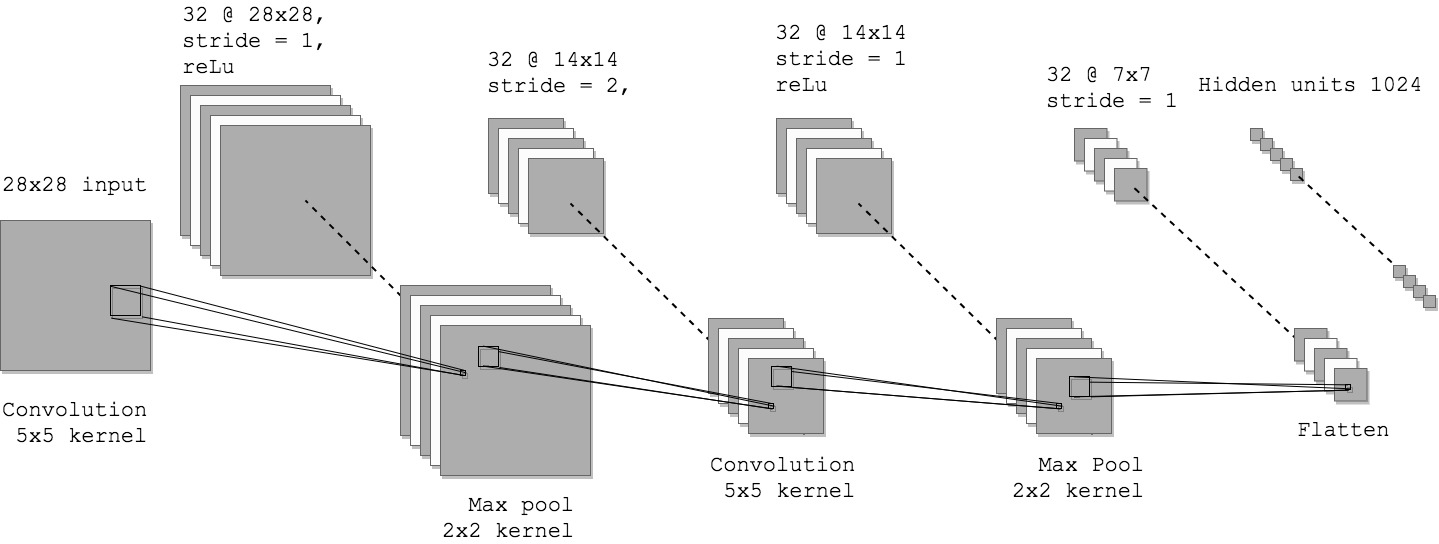
\includegraphics[width=1\linewidth]{../diagrams/MNIST_network}
\caption{Training set:55,000. Test set: 10,000. Training error: 2.4 \%. Test error: 2.79 \%. Total training time: 91 seconds}
\label{fig:mnistnetwork}
\end{figure}


\pagebreak

As before, we visualize some weights directly.

\begin{figure}[h]
\centering
\includegraphics[width=0.7\linewidth]{../../../../../../../Desktop/weights_mnist2}
\caption{Random subset of filter weights}
\label{fig:weightsmnist2}
\end{figure}

\begin{figure}[h]
\centering
\includegraphics[width=0.7\linewidth]{../../../../../../../Desktop/weights_mnist1}
\caption{Random subset of filter weights}
\label{fig:weightsmnist1}
\end{figure}




Weight projection, for this dataset and network, is not nearly as informative as it was for EFL. Although there is some semblance of structure to the positive and negative weights, any comment on its significance is most likely a stretch. Furthermore, the mapping performed by the convolutional layer is not one-to-one, so we expect non-interpretable filter weights. As a consequence, it is reasonable for all subsequent weights to be visually non-interpretable. \\


Feature-map visualization may give us further insight onto what this slightly more complex network has learned. As explained above, we can plot stored activation for each neuron in our network. We choose to focus on a subset of the most "important" nodes. \\

The question of which nodes are most "important" is non-trivial, so as a first approximation we selected the three highest activations across all test-set images for three random nodes per layer. We modify the activation definitions in (Lengerich et al., 2017) \cite{resampling} and (Koman, 2017) \cite{koman} in favor of the square norm of the feature map after each subsequent kernel instead of summing over all elements. Formally,

\begin{align*}
	z(l, i, j) = ||\delta_j^{l-1} * w_{i}^l||_F\\
\end{align*}

Where $\delta_j^{l - 1}$ is the signal emitted by the previous layer after passing the $j th$ image, * is the convolutional operation with $w_i^l$ weights in the $i$th filter and $l$th layer. This is not a vector norm but the Frobenius norm defined by: \\

\begin{align*}
	||A||_F = \sqrt{\sum_{i = 1}^{m} \sum_{j = 1}^{n} |a_{i,j}|^2}
\end{align*}

A more subtle approach at identifying the relationship between a neuron and input is through deconvolutional neural networks (deconvnet) (Zeiler, 2013)\cite{zeiler}. Much like an auto-encoder, a deconvnet attempts to recover the original data input from an intermediate layer. In other words, it projects hidden activations back to pixel-space, a problem first described by (Erhan et al., 2009) \cite{bengio}. Some possible advantages of deconvnet over visualizing hidden activations directly is that we can visualize layers of very dissimilar dimension to the input (and of decaying resolution) and that we recover some spatial specificity in the pixel-space. The steps to deconvolving are \\

i) Unpooling: Assigning maximum values to saved maximum locations (or switches). All other locations are zero. We follow the modification BY KVFRANS AND OXFORD to assign the maximum to the entire filter location. Saving switch locations was very computationally expensive. \\

ii) UnRelu: Passing the reLu function once more. \\

iii) Deconvolution: Apply a convolution with equal filter-size but the transpose of already trained weights. \\

Below we add the figure from (Zeiler et al., 2013) that diagrams deconvnet architecture. Notice that the network's architecture changes for deeper layers of interest as the number of operations necessary to project back to pixel-space grows. \\

\begin{figure} [H]
	\centering
	\includegraphics[width=0.7\linewidth]{../../../../../../../Desktop/zeiler_deconv}
	\caption{Training set:}
	\label{fig:zeilerdeconv}
\end{figure}

We follow the above selection criteria: randomly select 3 nodes within each layer and find the top-3 activation images for each within the test-set. Below we show the input image, feature-map visualization and deconvolutional projection. We organize the images by node, showing, from top to bottom, input image,  feature map visualization and deconvolutional projection.

\begin{center}
	\begin{figure}[H]
		\centering
		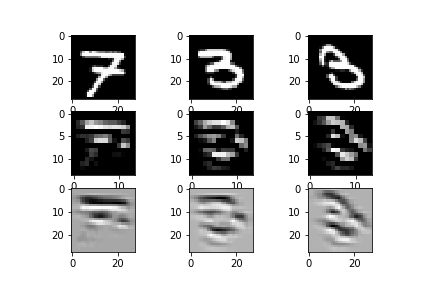
\includegraphics[width=0.6\linewidth]{../diagrams/node1_layer1_mnist}
		\caption{Node 1, Layer 1}
		\label{fig:node1layer1mnist}
	\end{figure}
	\begin{figure}[H]
		\centering
		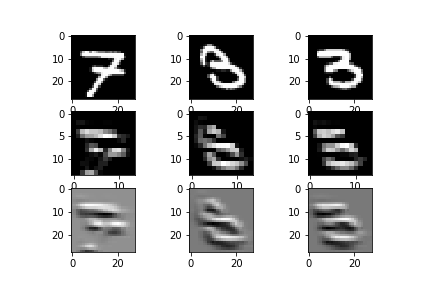
\includegraphics[width=0.6\linewidth]{../diagrams/node16_layer1_mnist}
		\caption{Node 16, Layer 1}
		\label{fig:node16layer1mnist}
	\end{figure}
	\pagebreak
	\begin{figure}[H]
		\centering
		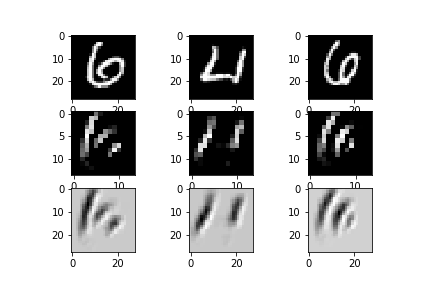
\includegraphics[width=0.6\linewidth]{../diagrams/node22_layer1_mnist}
		\caption{Node 22, Layer 1}
		\label{fig:node22layer1mnist}
	\end{figure}
		\begin{figure}[H]
			\centering
			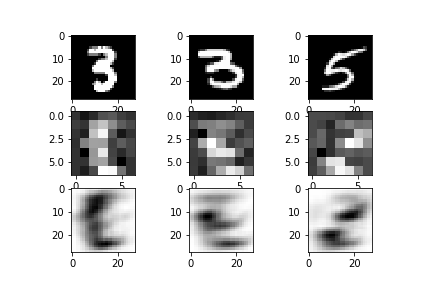
\includegraphics[width=0.6\linewidth]{../diagrams/node3_layer2_mnist}
			\caption{Node 3, Layer 2}
			\label{fig:node3layer2mnist}
		\end{figure}
	\begin{figure}[H]
		\centering
		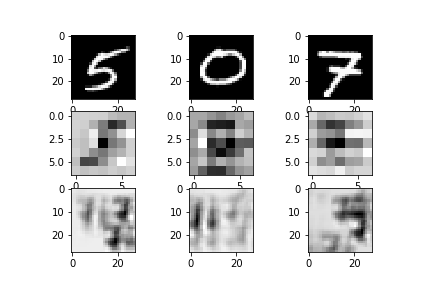
\includegraphics[width=0.6\linewidth]{../diagrams/node32_layer2_mnist}
		\caption{Node 32, Layer 2}
		\label{fig:node32layer2mnist}
	\end{figure}
	\begin{figure}[H]
		\centering
		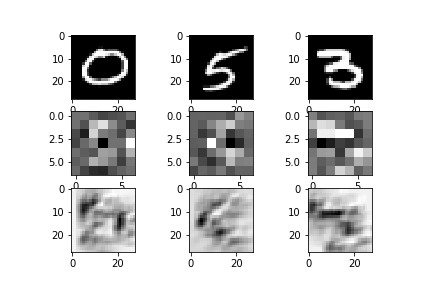
\includegraphics[width=0.6\linewidth]{../diagrams/node45_layer2_mnist}
		\caption{Node 45, Layer 2}
		\label{fig:node45layer2mnist}
	\end{figure}
\end{center}

Our first observation is that each filter has developed unique characteristics and produces visually consistent activations across all the visualized inputs. For instance, node 1 in layer 1 (\textit{Figure 11})  is maximally activated by horizontal features, while node 22 in the same layer \textit{Figure 13} fires with diagonal strokes. Node 16 in layer 1 \textit{Figure 12} also appears to prefer horizontal features, although its respective images are definitely not identical to node 1's. Accordingly, the top-3 activation images are the same the same for both nodes, although in different rank order.  \\

Furthermore, deconvolutions produce clearer images than weight visualization as we go deeper into the network. However, the projections of our nodes within layer two do not appear to have an obvious interpretation. Nonetheless, each node continues to be visually consistent.

\subsubsection{Input optimization}

In some respect, the above selection procedure optimizes for maximum activation across the entire test set for a single node. We can express this as:

\[
X^* = \arg \max_{x_j\in X} (z(l, i, j))
\]

Where $x_j$ it the $j$th image in the X dataset.

\section{Dog, Muffin or Fried Chicken?}

MNIST, however, is still a fairly homogeneous dataset. We turn to the Dog, Muffin and Fried Chicken dataset to experiment with multi-channel feature visualization and a more complex network. In order to make the dataset more computationally tractable, we reduce the resolution so each image is 128x128 pixels. We therefore have three channels, three convolutional layers and one fully connected layer. As with most RGB images, we pre-process the input by dividing the maximum possible activation of each pixel (255). In addition, we expand the dataset by generating more images that are flipped and rotated versions of the original ones, conserving their labels. \\

\begin{figure} [H]
\centering
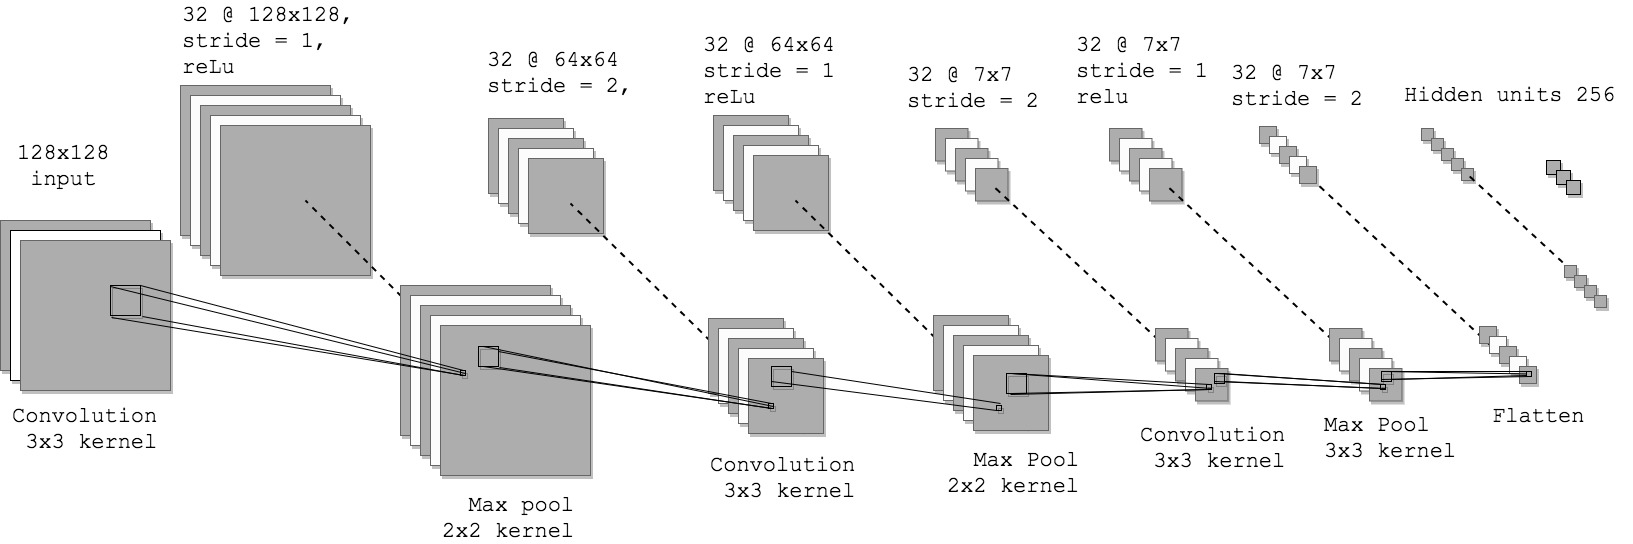
\includegraphics[width=1\linewidth]{../diagrams/DMC_network}
\caption{Training set: 8,071 (including rotated images). Test set: 896. Training error: 3.59 \%, Test error: 11.05 \%. Total training time: 924 seconds}
\label{fig:dmcnetwork}
\end{figure}

Repeating the procedure implemented in MNIST, except without visualizing weights since we expect no actionable information and fixing filter numbers. We have for nodes 8, 15 and 23 in every layer, their feature maps and the deconvnet visualization. As before, we show the input data, feature-map visualization and deconvolutional projection, from top to bottom.

\begin{figure} [H]
	\centering
	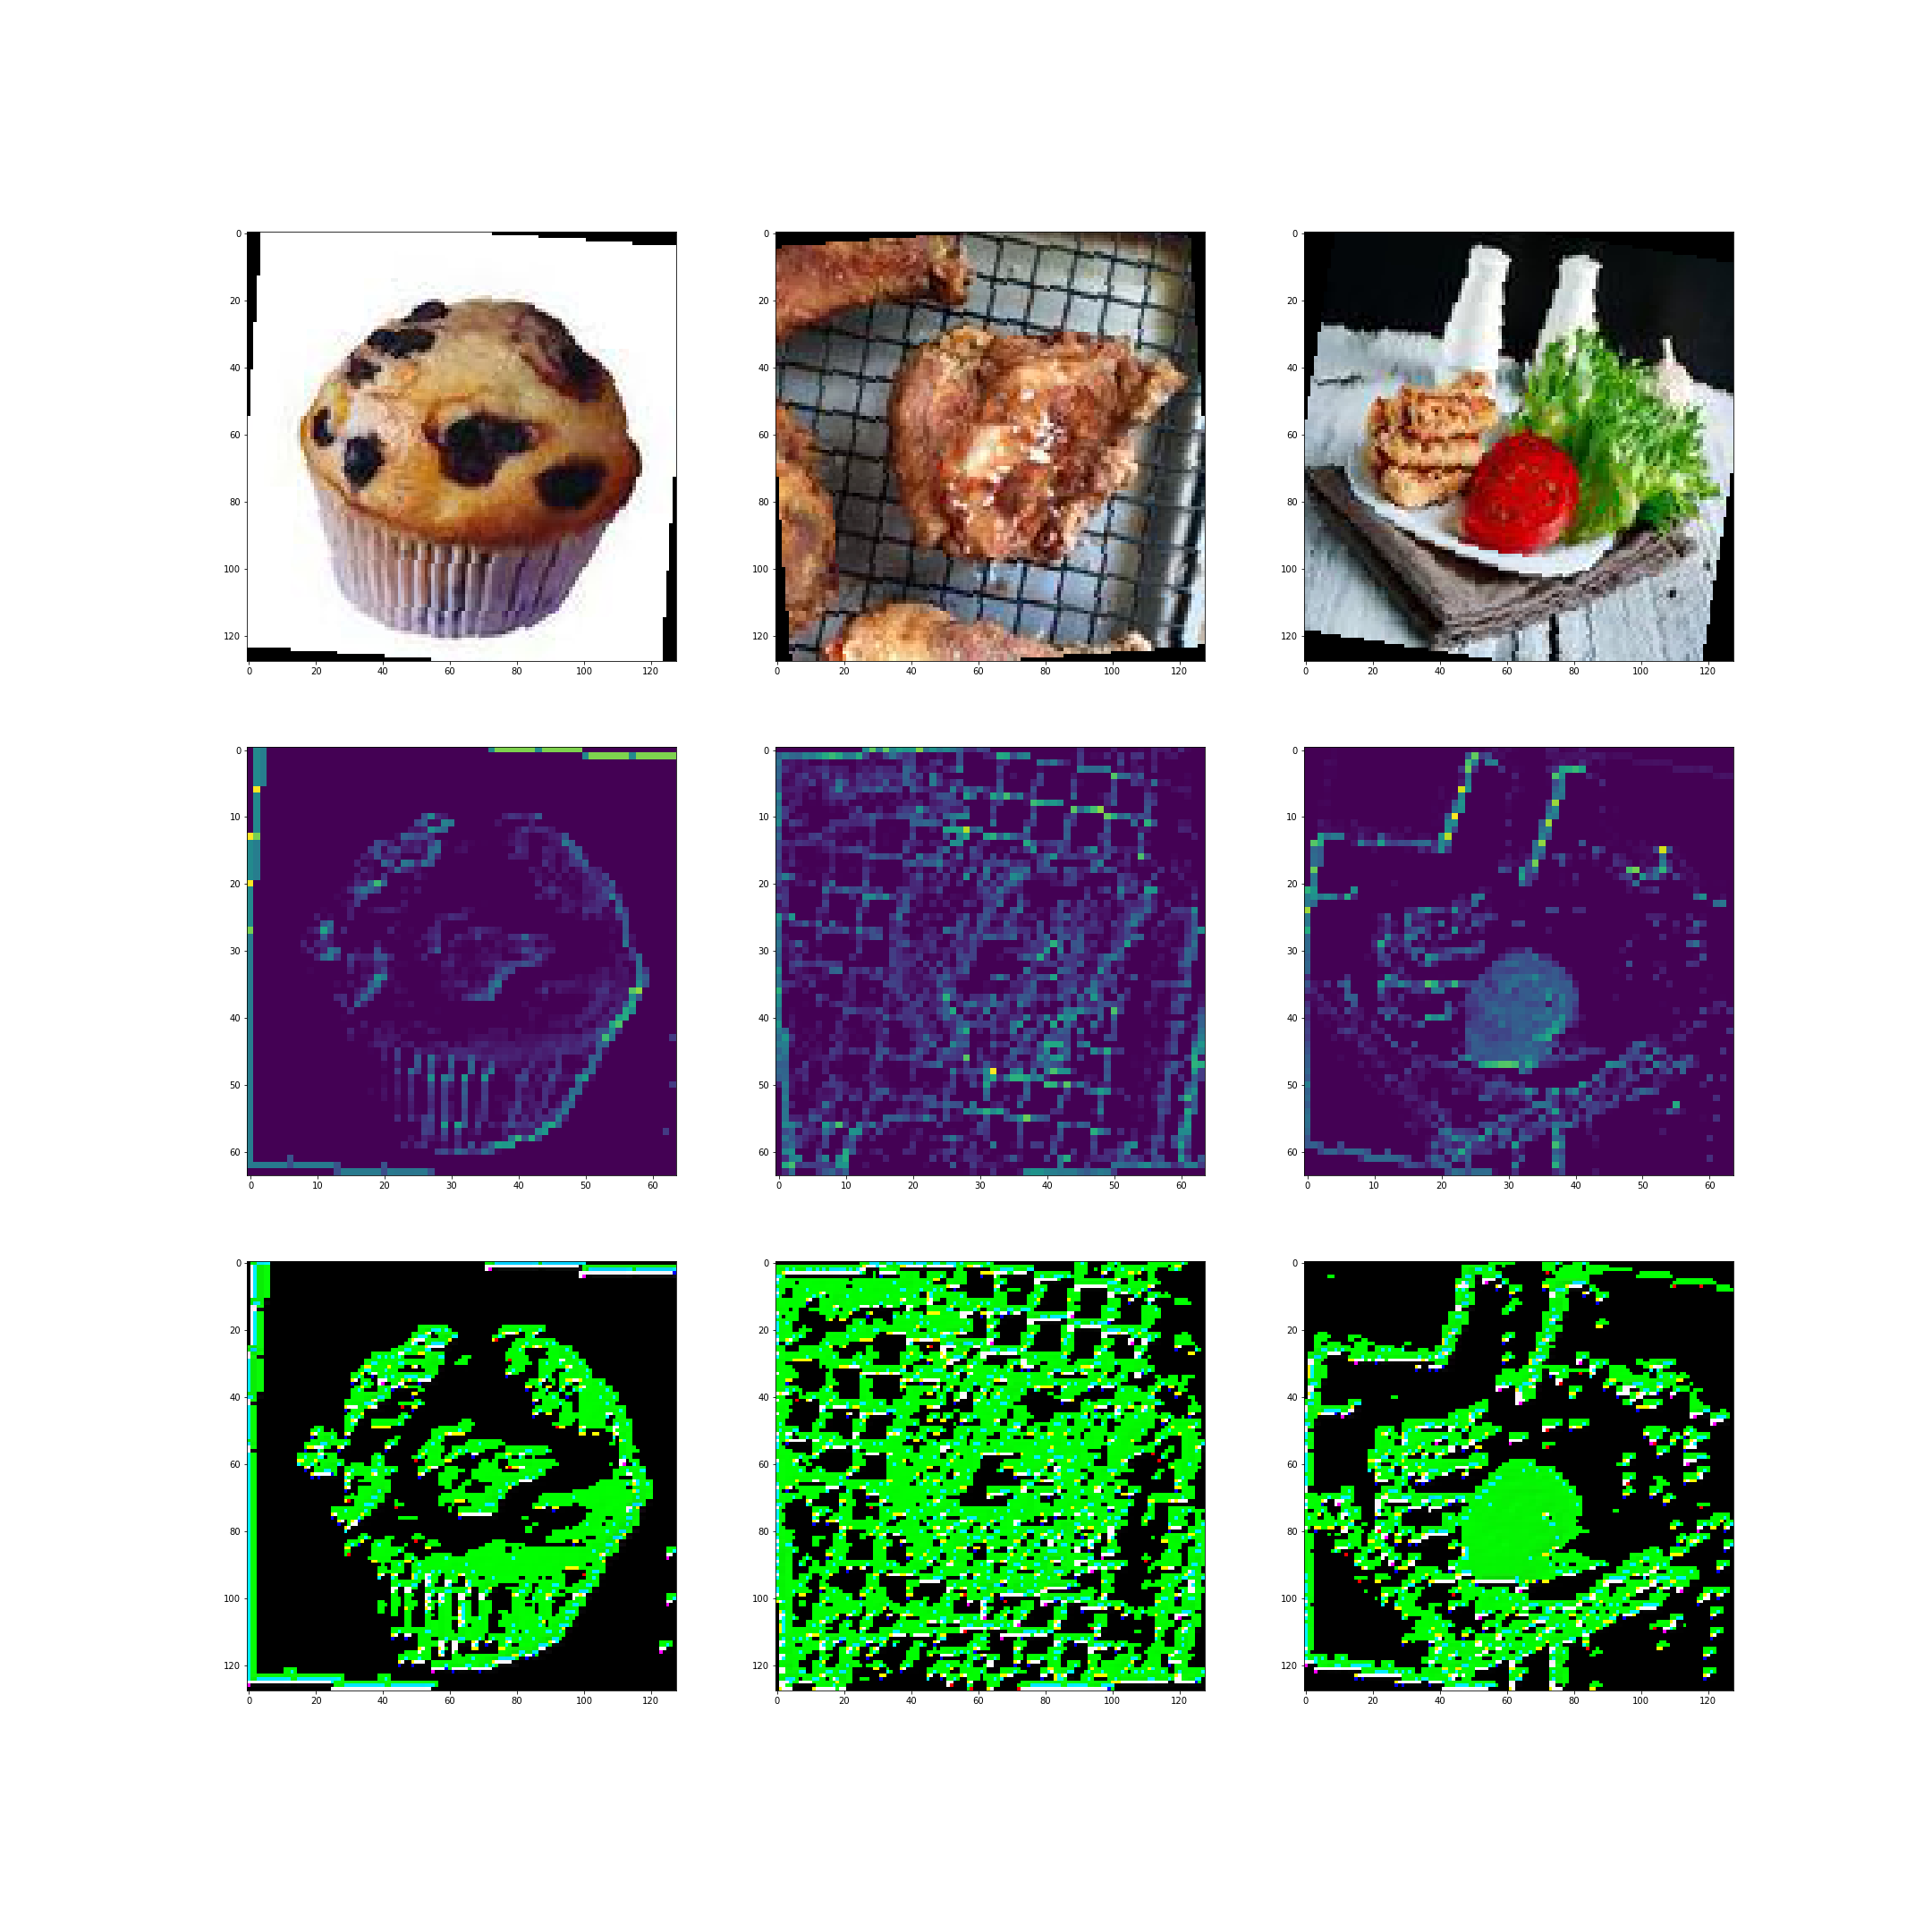
\includegraphics[width=0.7\linewidth]{../diagrams/node8_layer1_DMF}
	\caption{Node 8, Layer 1}
	\label{fig:node8layer1dmf}
\end{figure}
\begin{figure}[H]
	\centering
	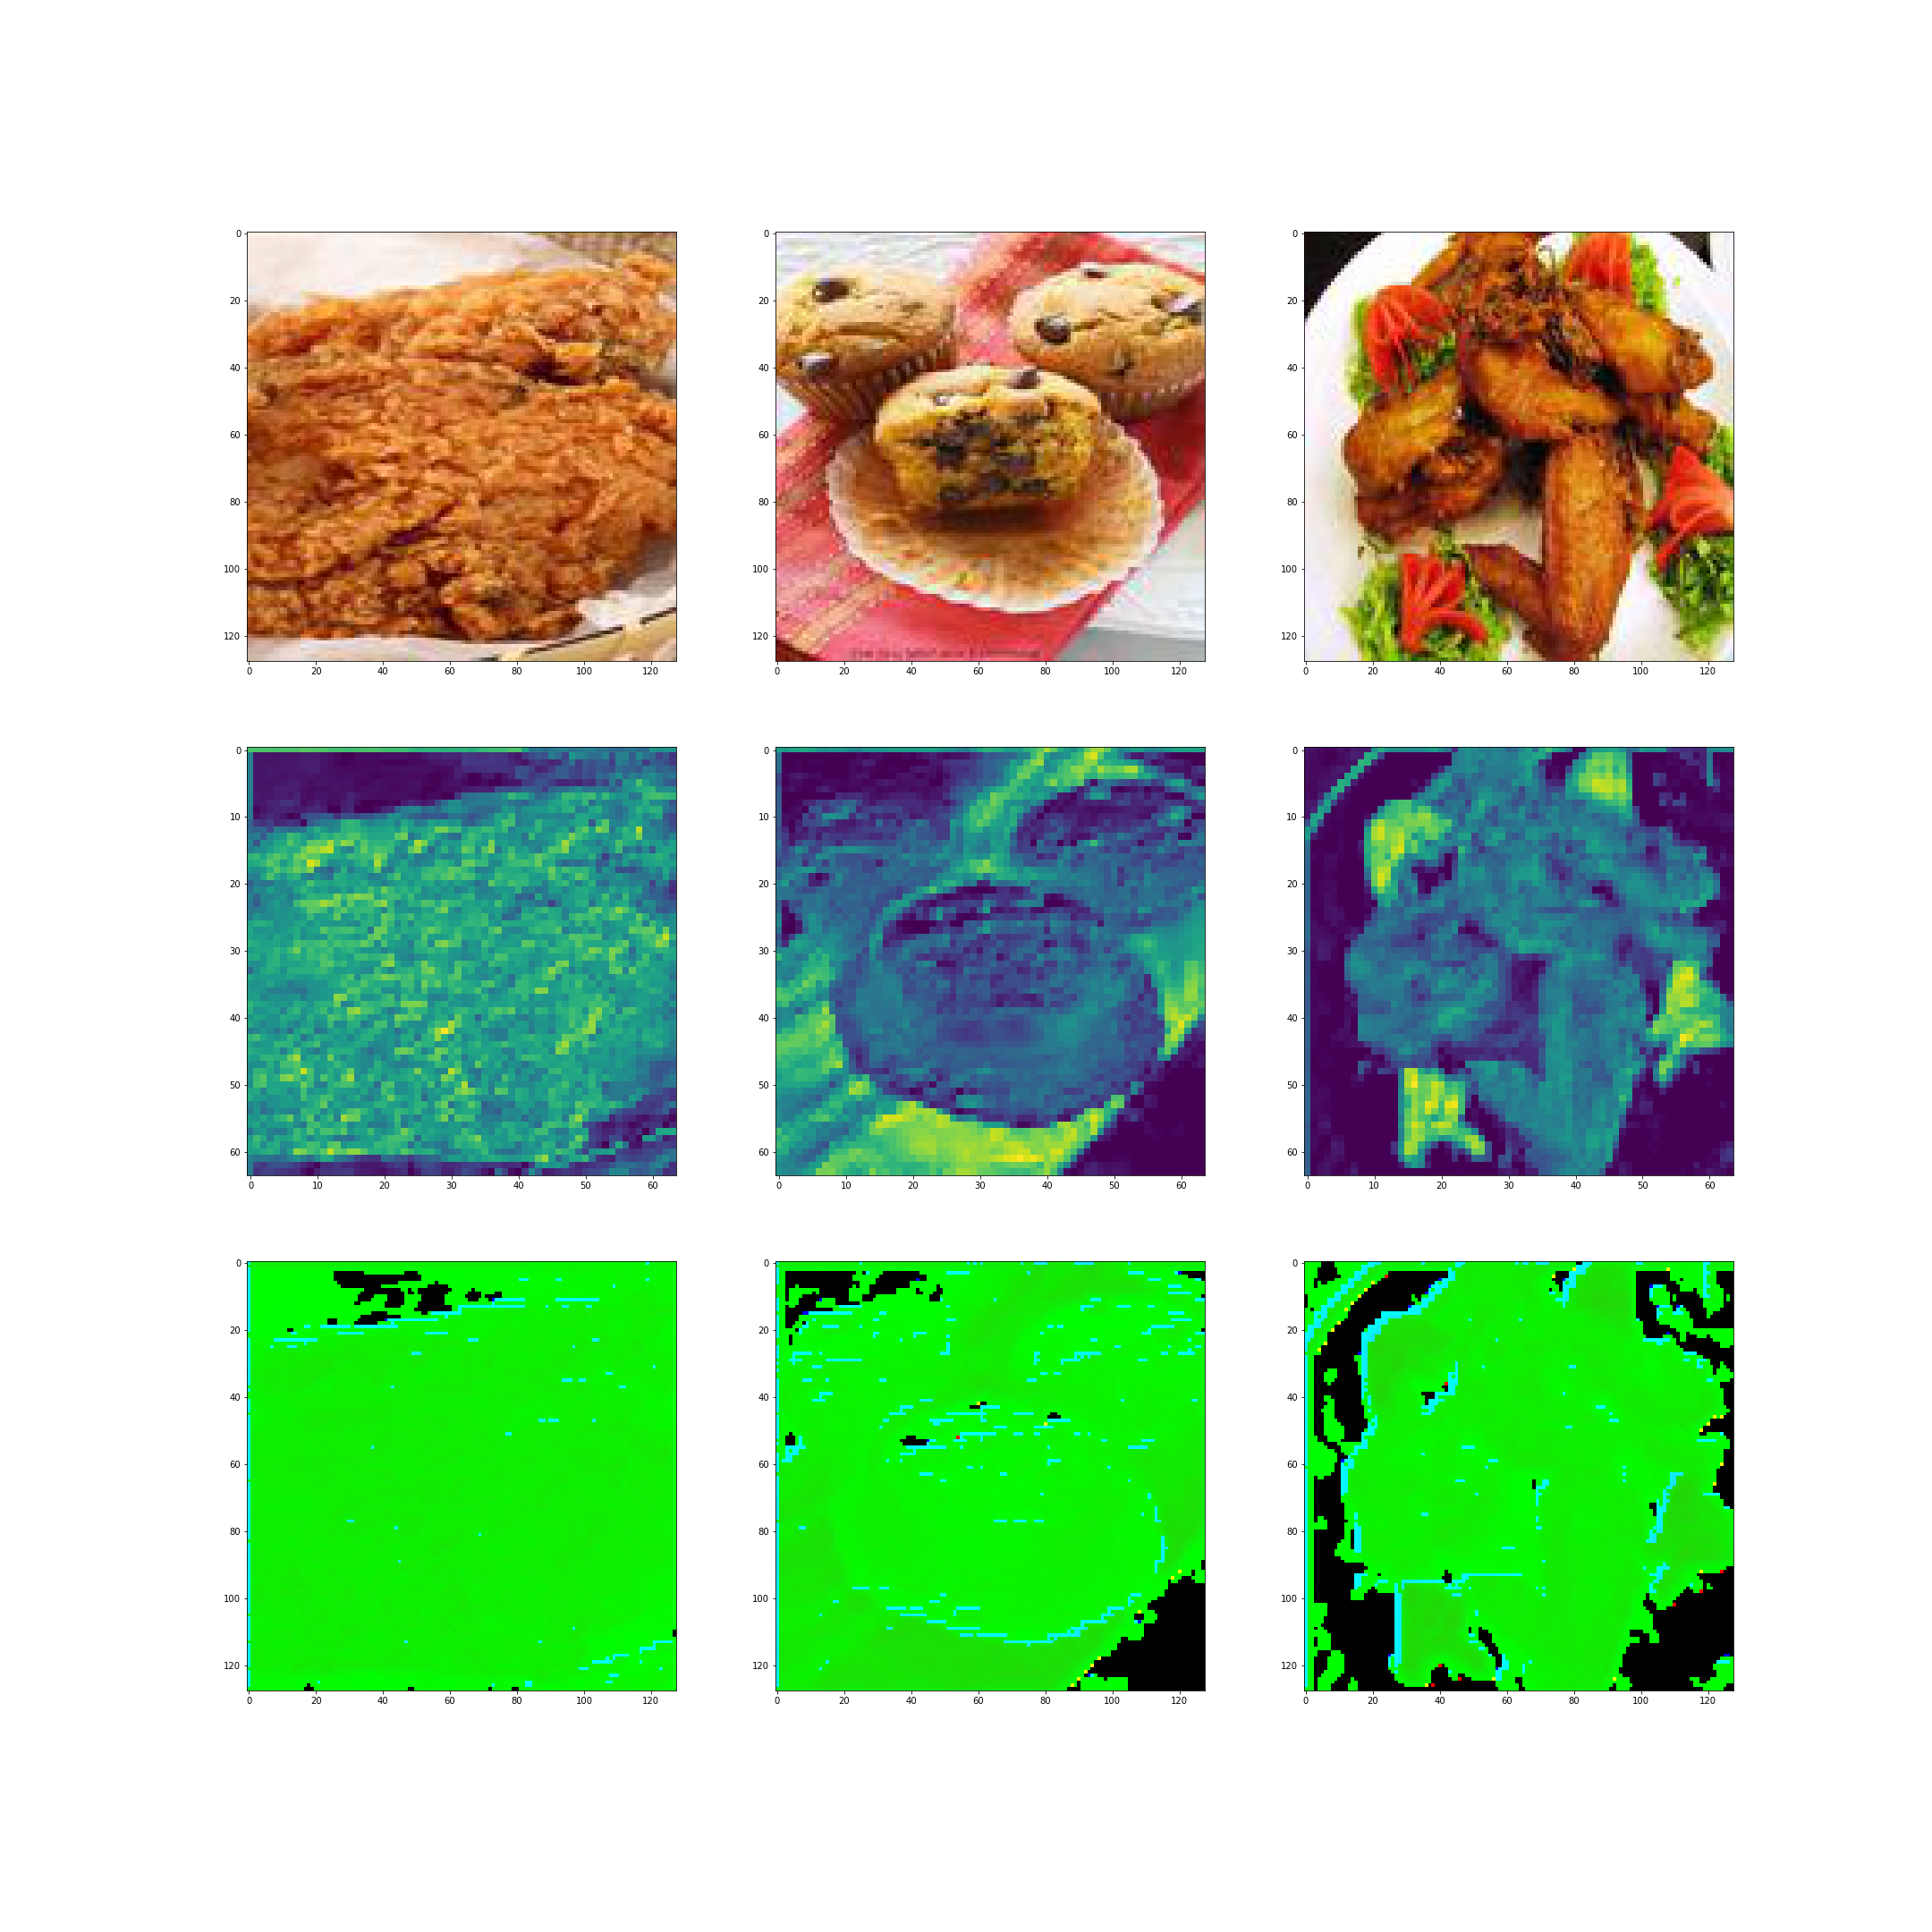
\includegraphics[width=0.7\linewidth]{../diagrams/node15_layer1_DMF}
	\caption{Node 15, Layer 1}
	\label{fig:node15layer1dmf}
\end{figure}
\begin{figure}[H]
	\centering
	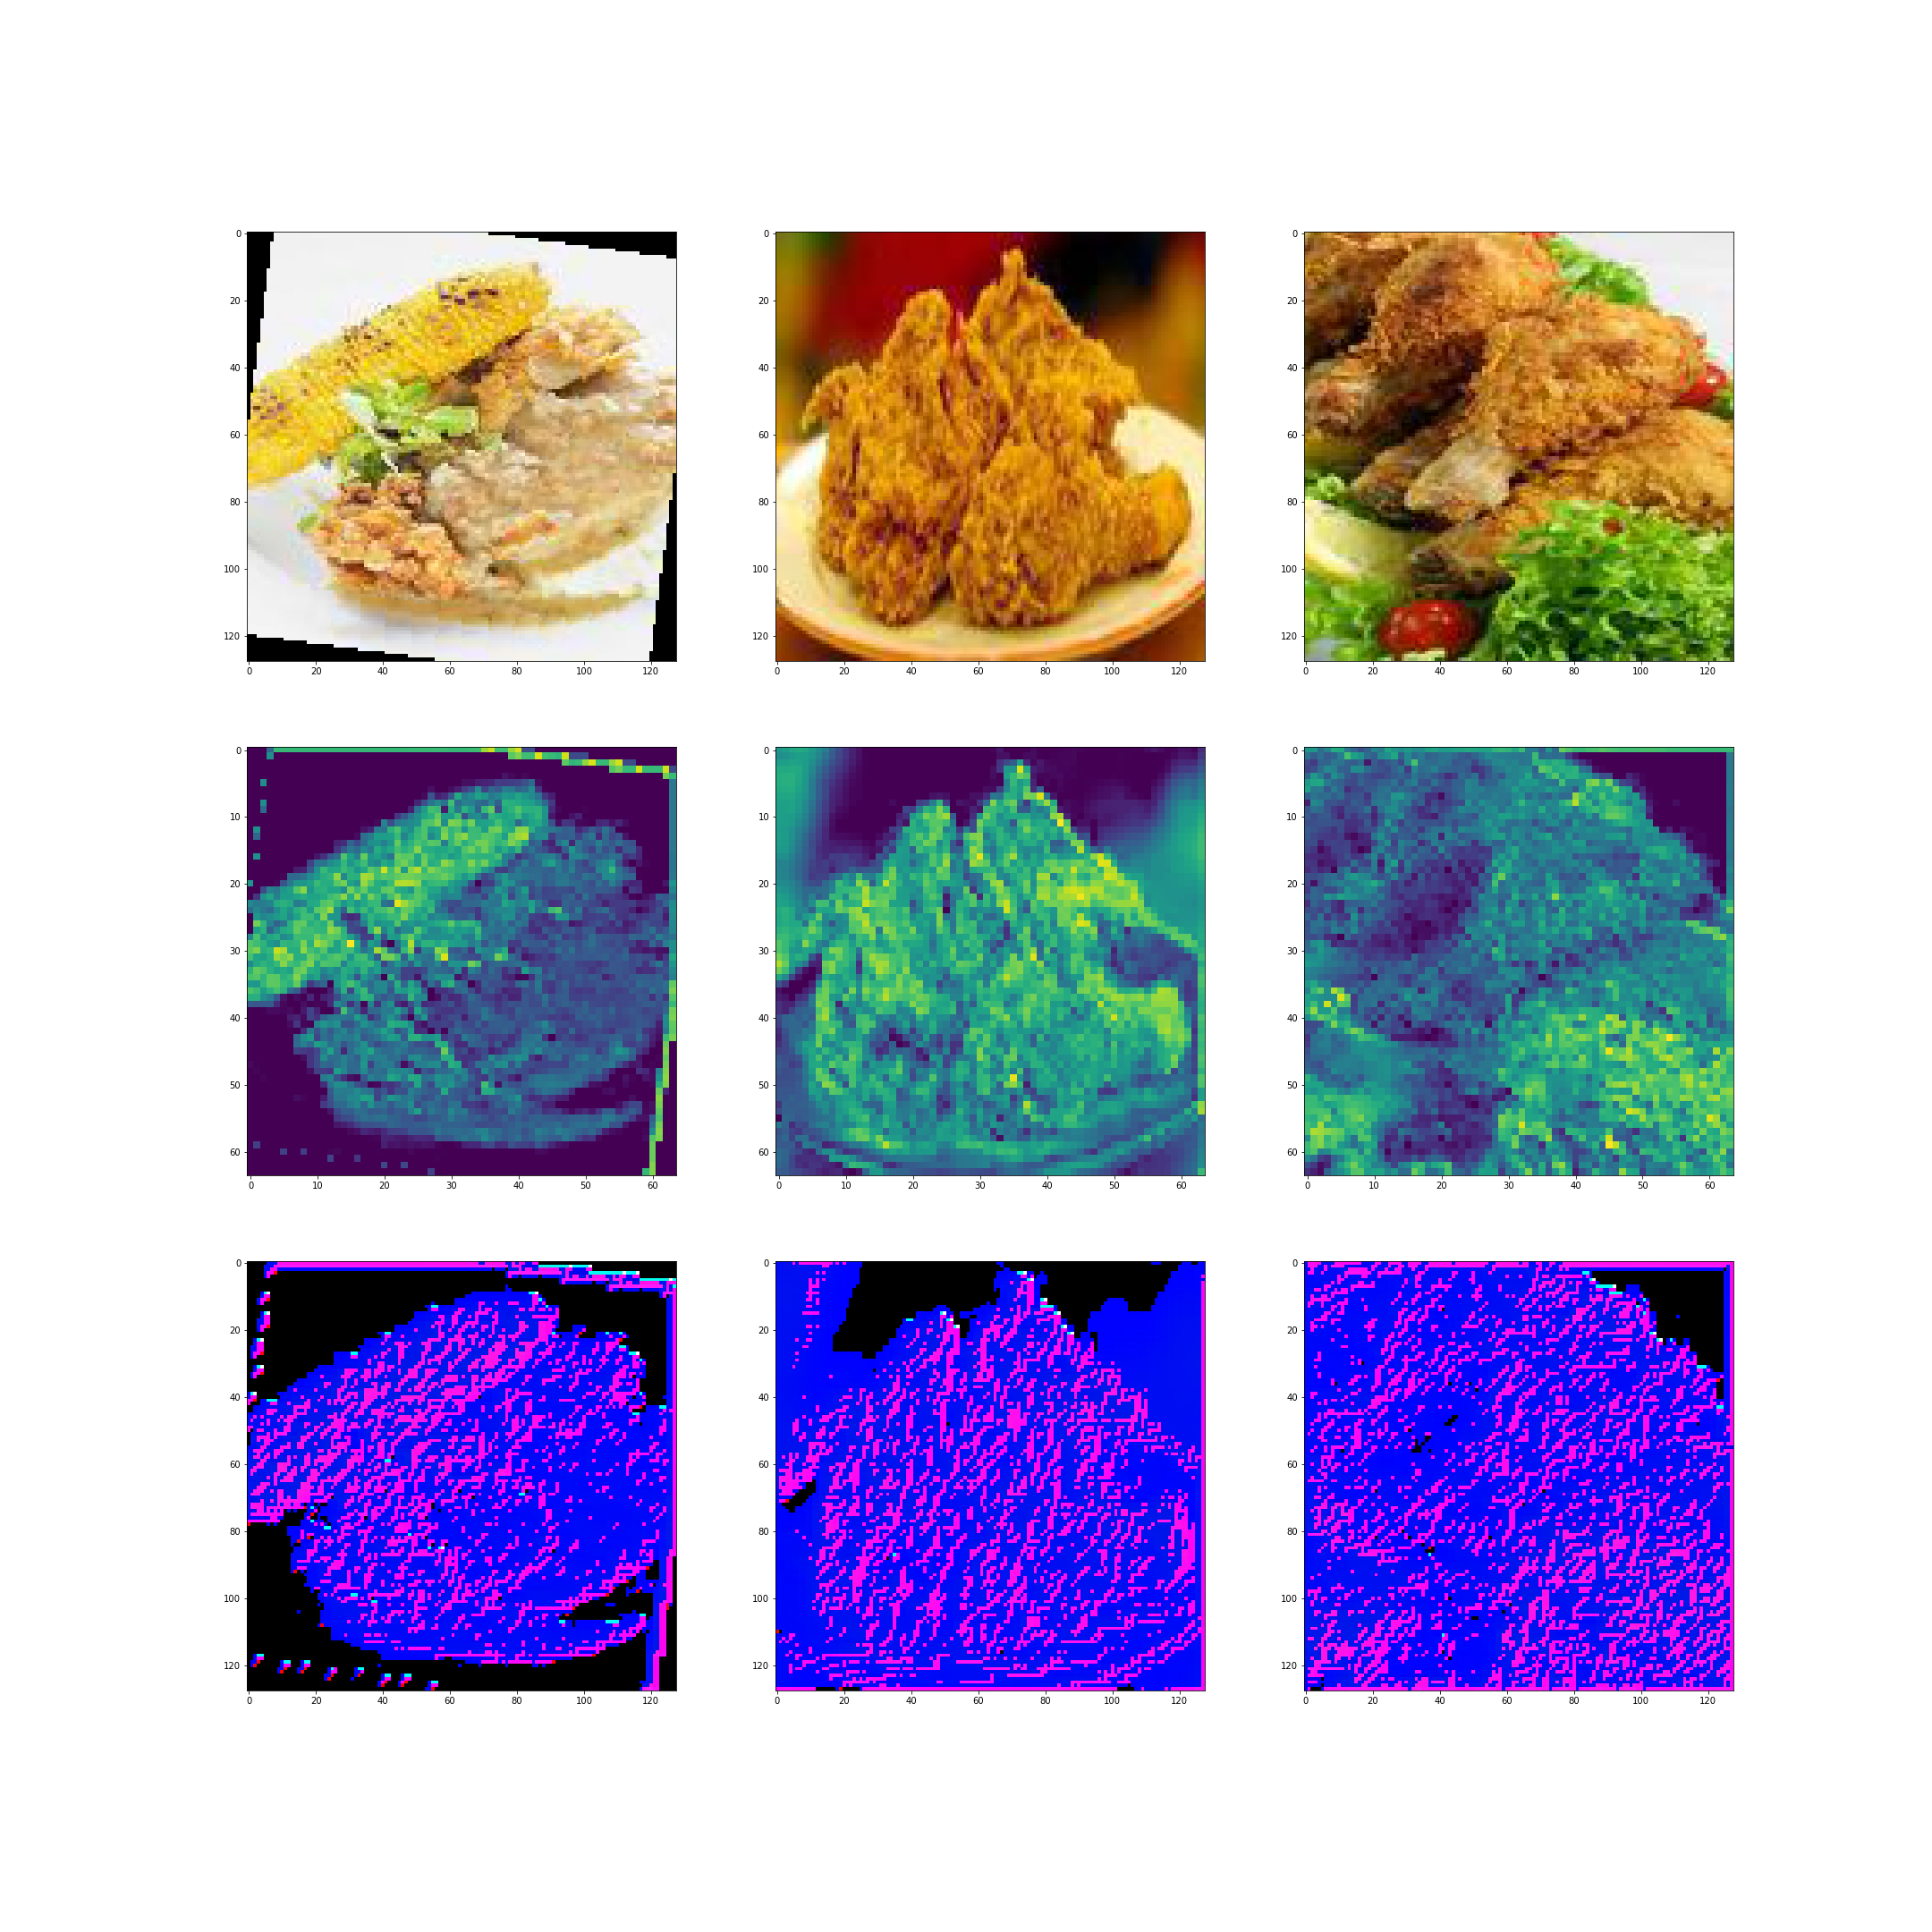
\includegraphics[width=0.7\linewidth]{../diagrams/node23_layer1_DMF}
	\caption{Node 23, Layer 1}
	\label{fig:node23layer1dmf}
\end{figure}
\begin{figure}[H]
	\centering
	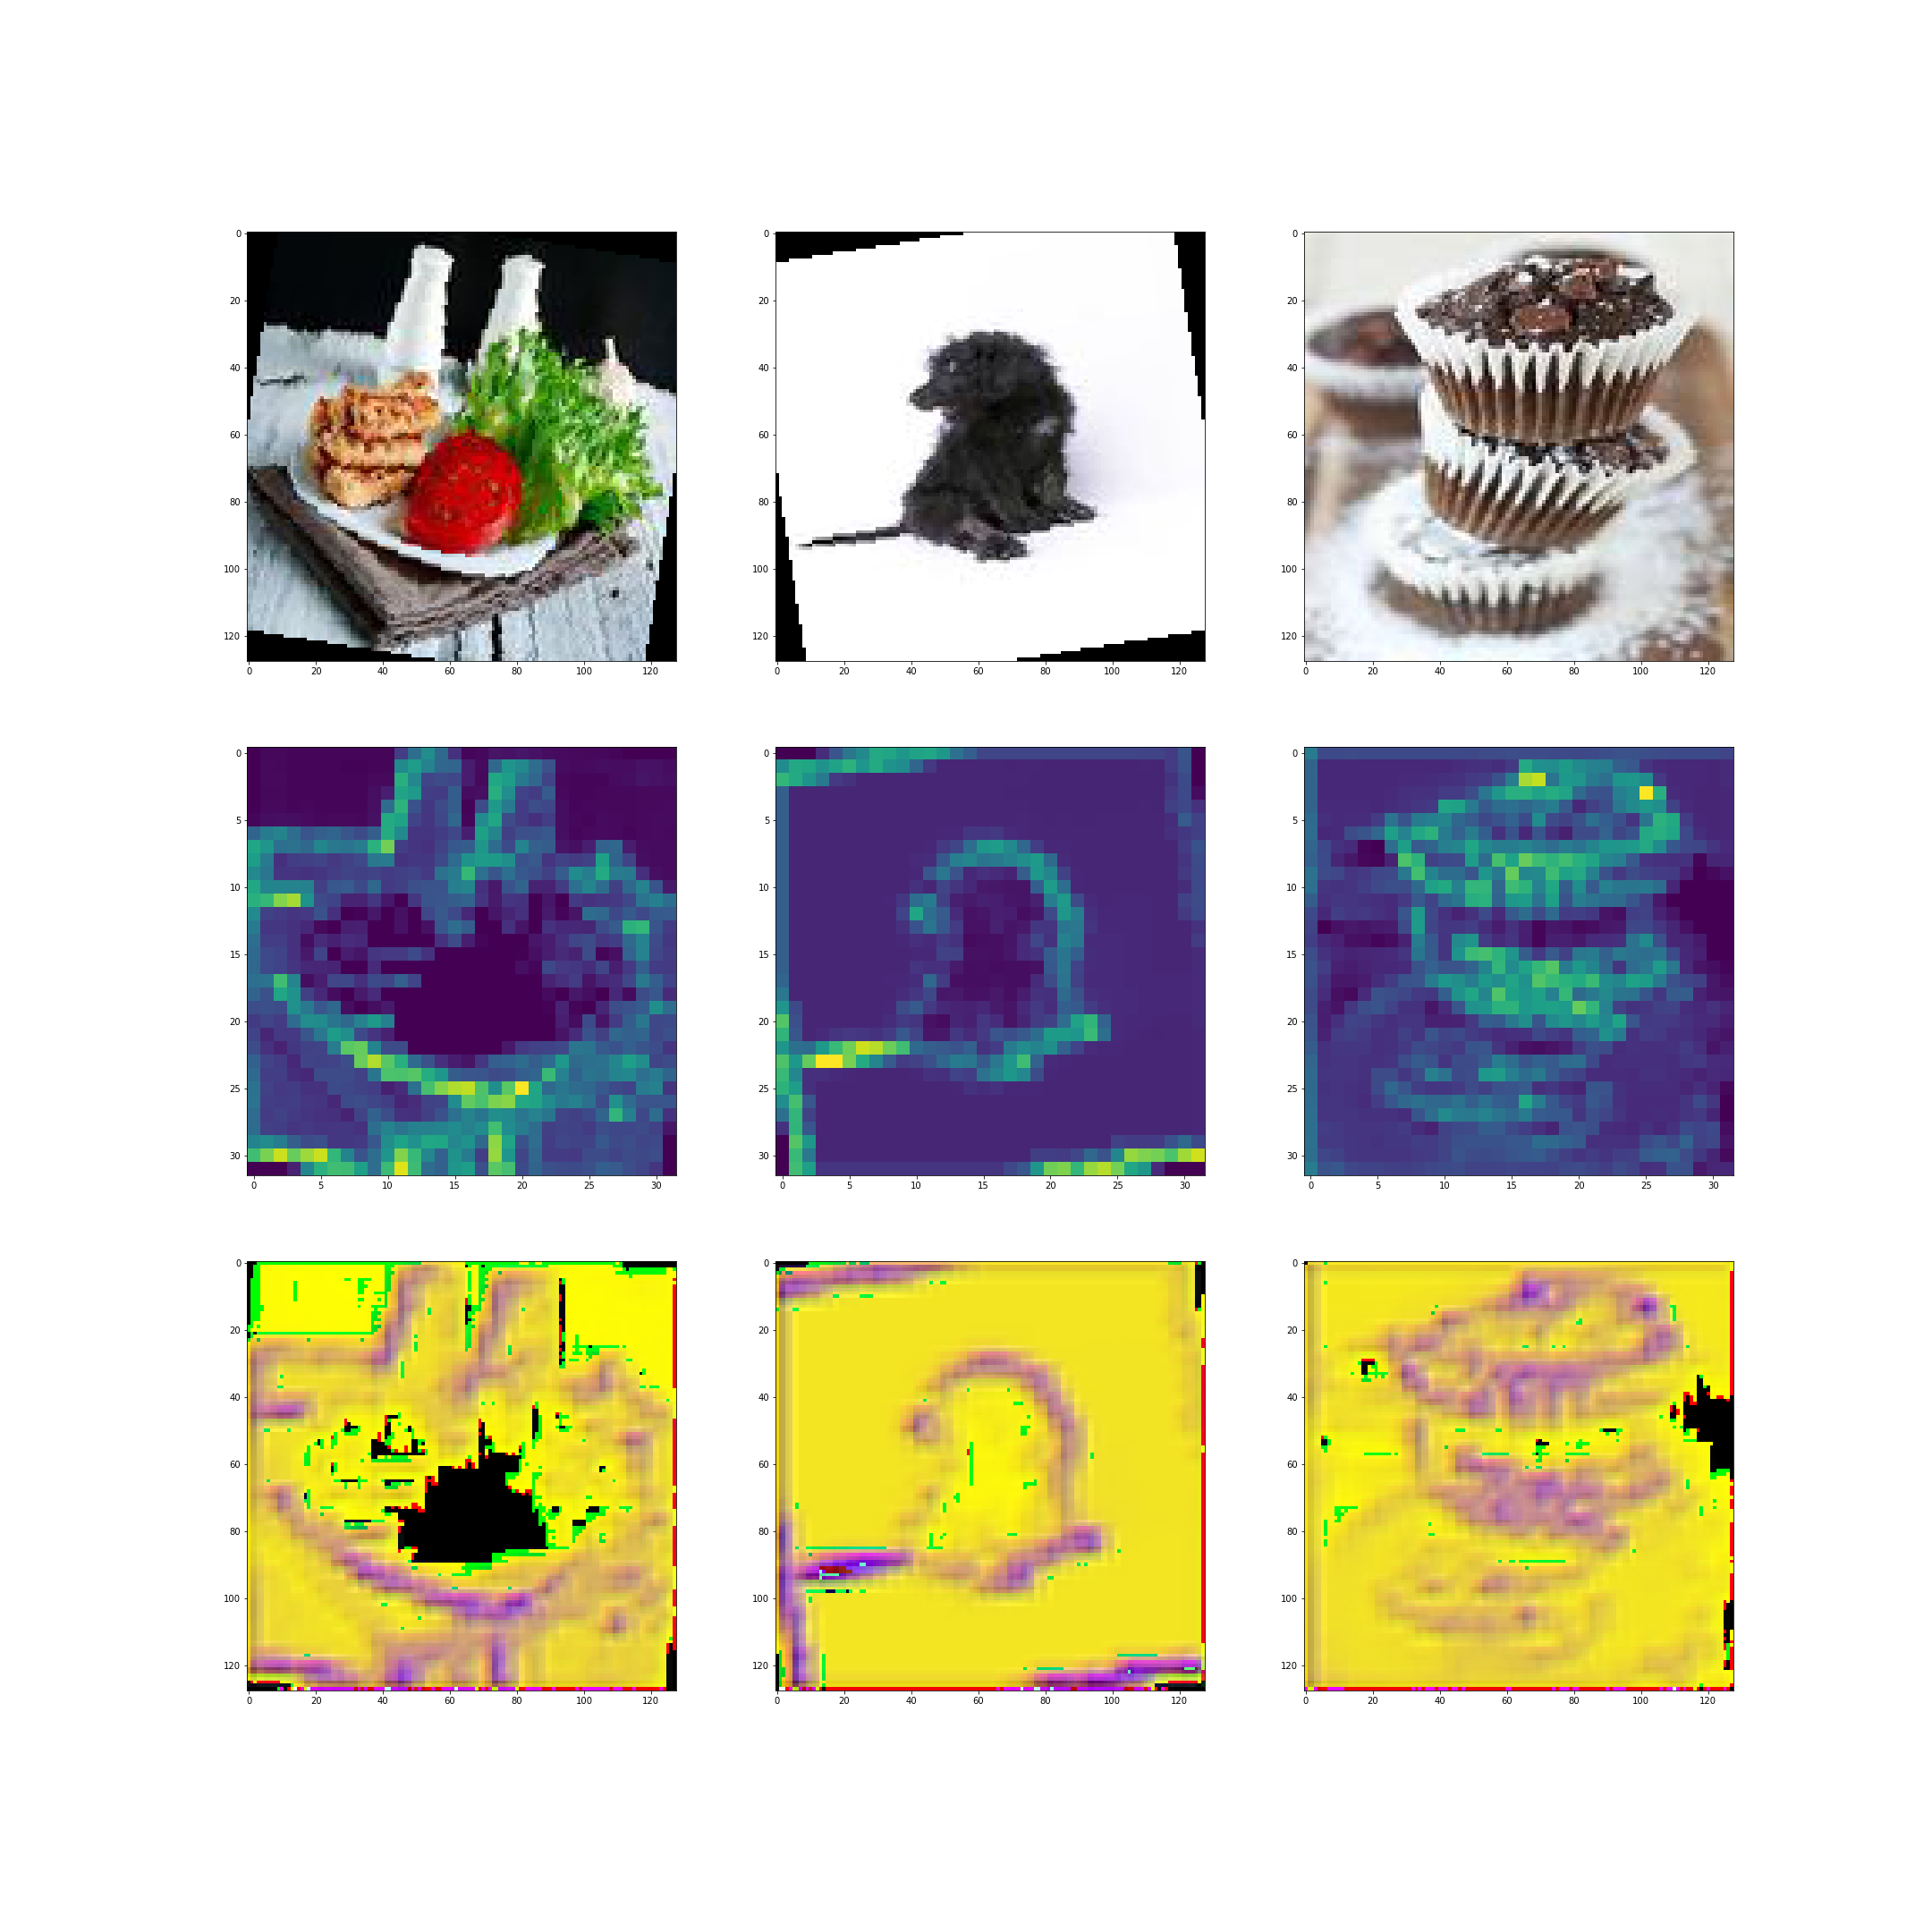
\includegraphics[width=0.7\linewidth]{../diagrams/node8_layer2_DMF}
	\caption{Node 8, Layer 2}
	\label{fig:node8layer2dmf}
\end{figure}
\begin{figure}
\centering
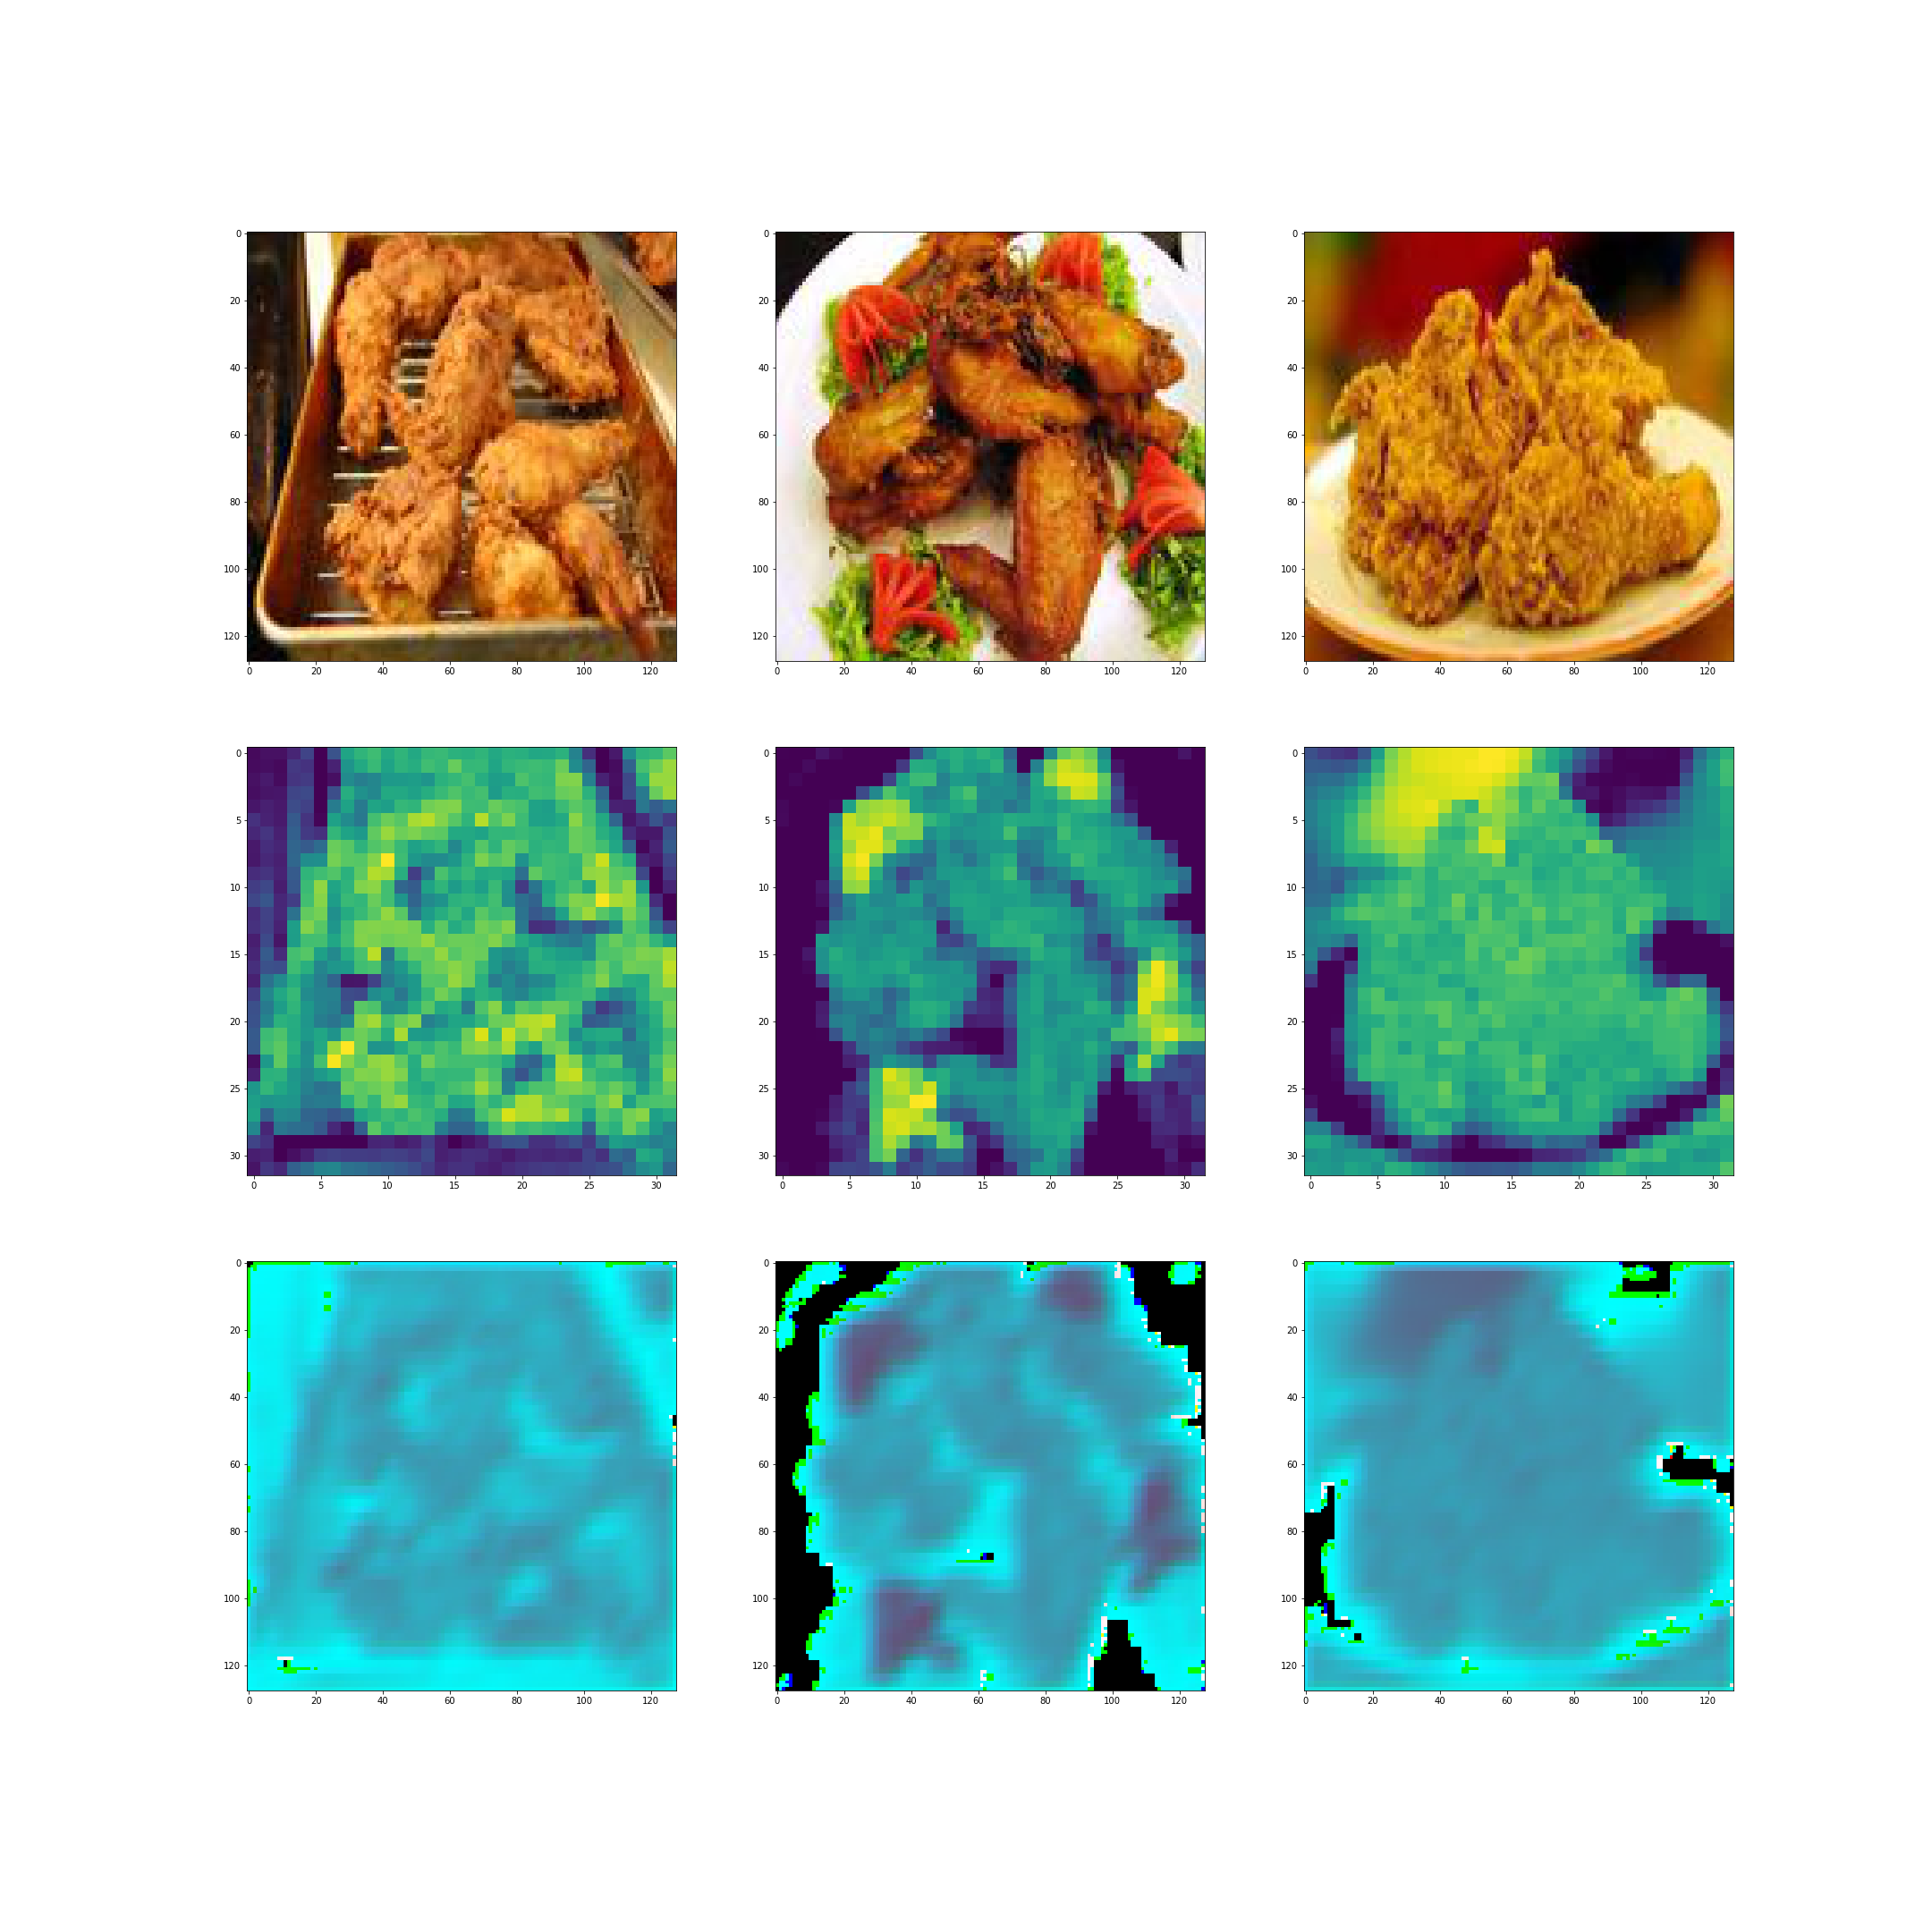
\includegraphics[width=0.7\linewidth]{../diagrams/node15_layer2_DMF}
\caption[Node 15, Layer 2]{}
\caption{}
\label{fig:node15layer2dmf}
\end{figure}
\begin{figure}[H]
	\centering
	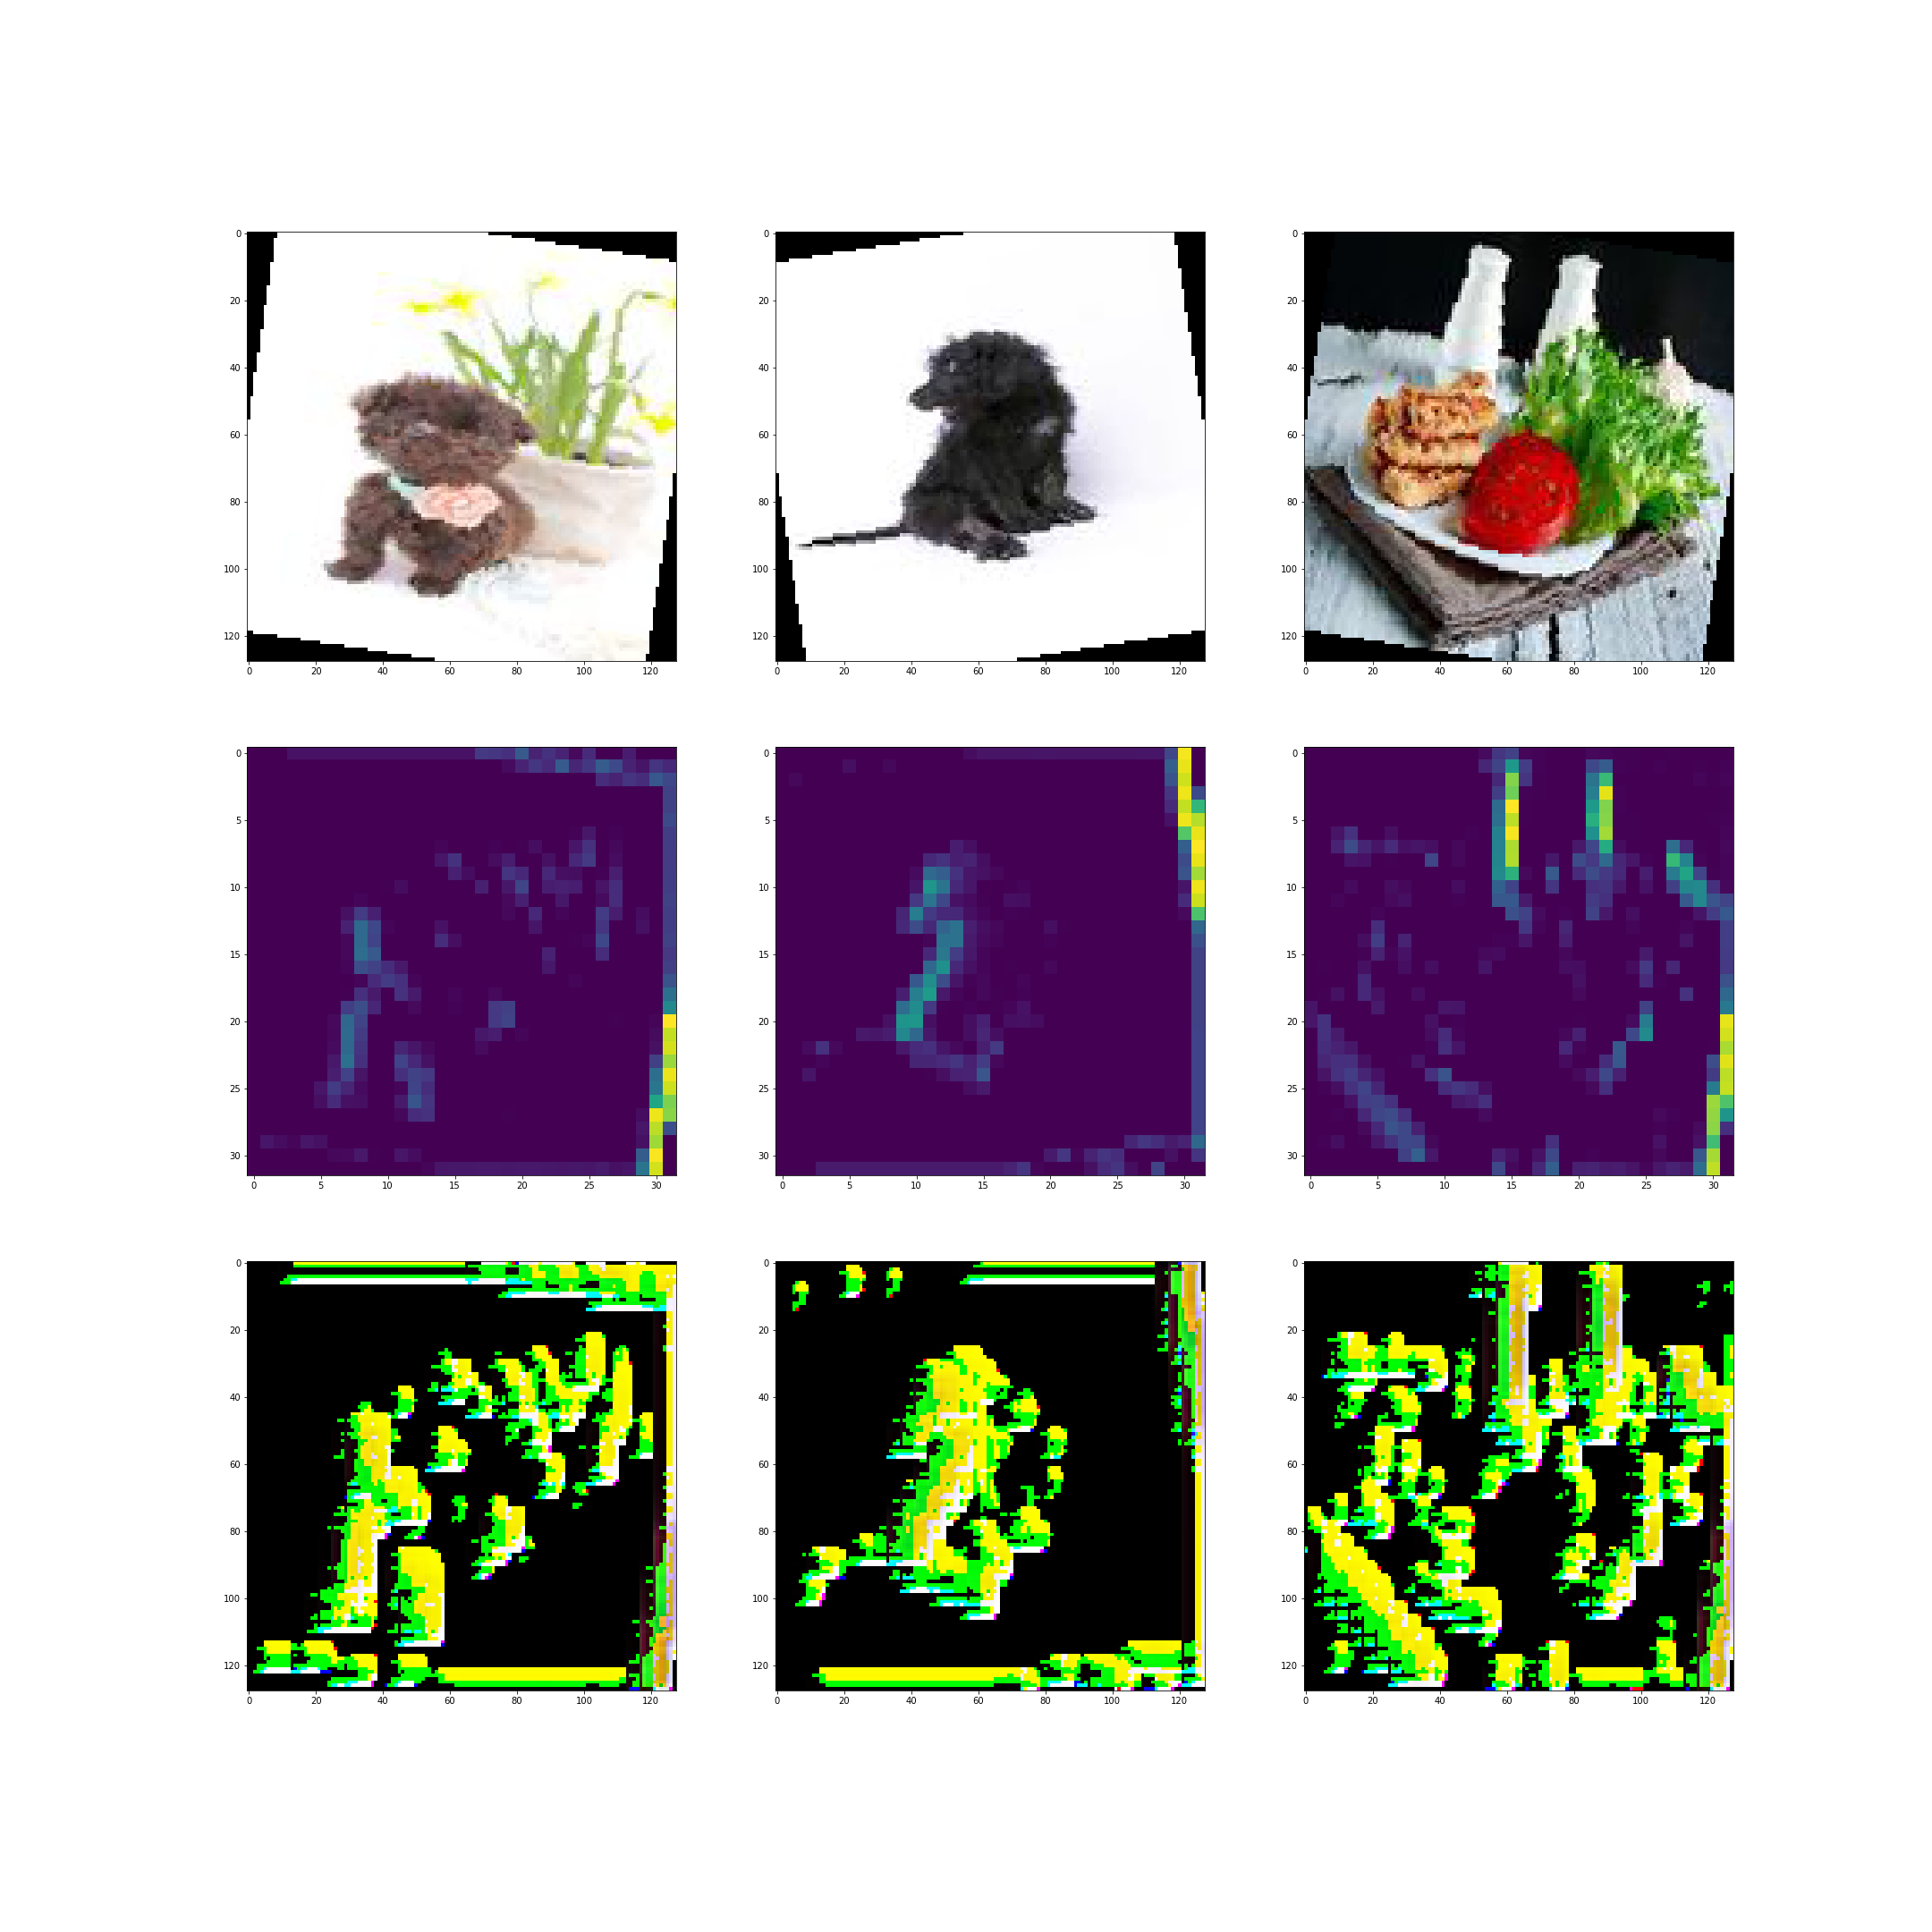
\includegraphics[width=0.7\linewidth]{../diagrams/node23_layer2_DMF}
	\caption{Node 23, Layer 2}
	\label{fig:node23layer2dmf}
\end{figure}
\begin{figure}[H]
	\centering
	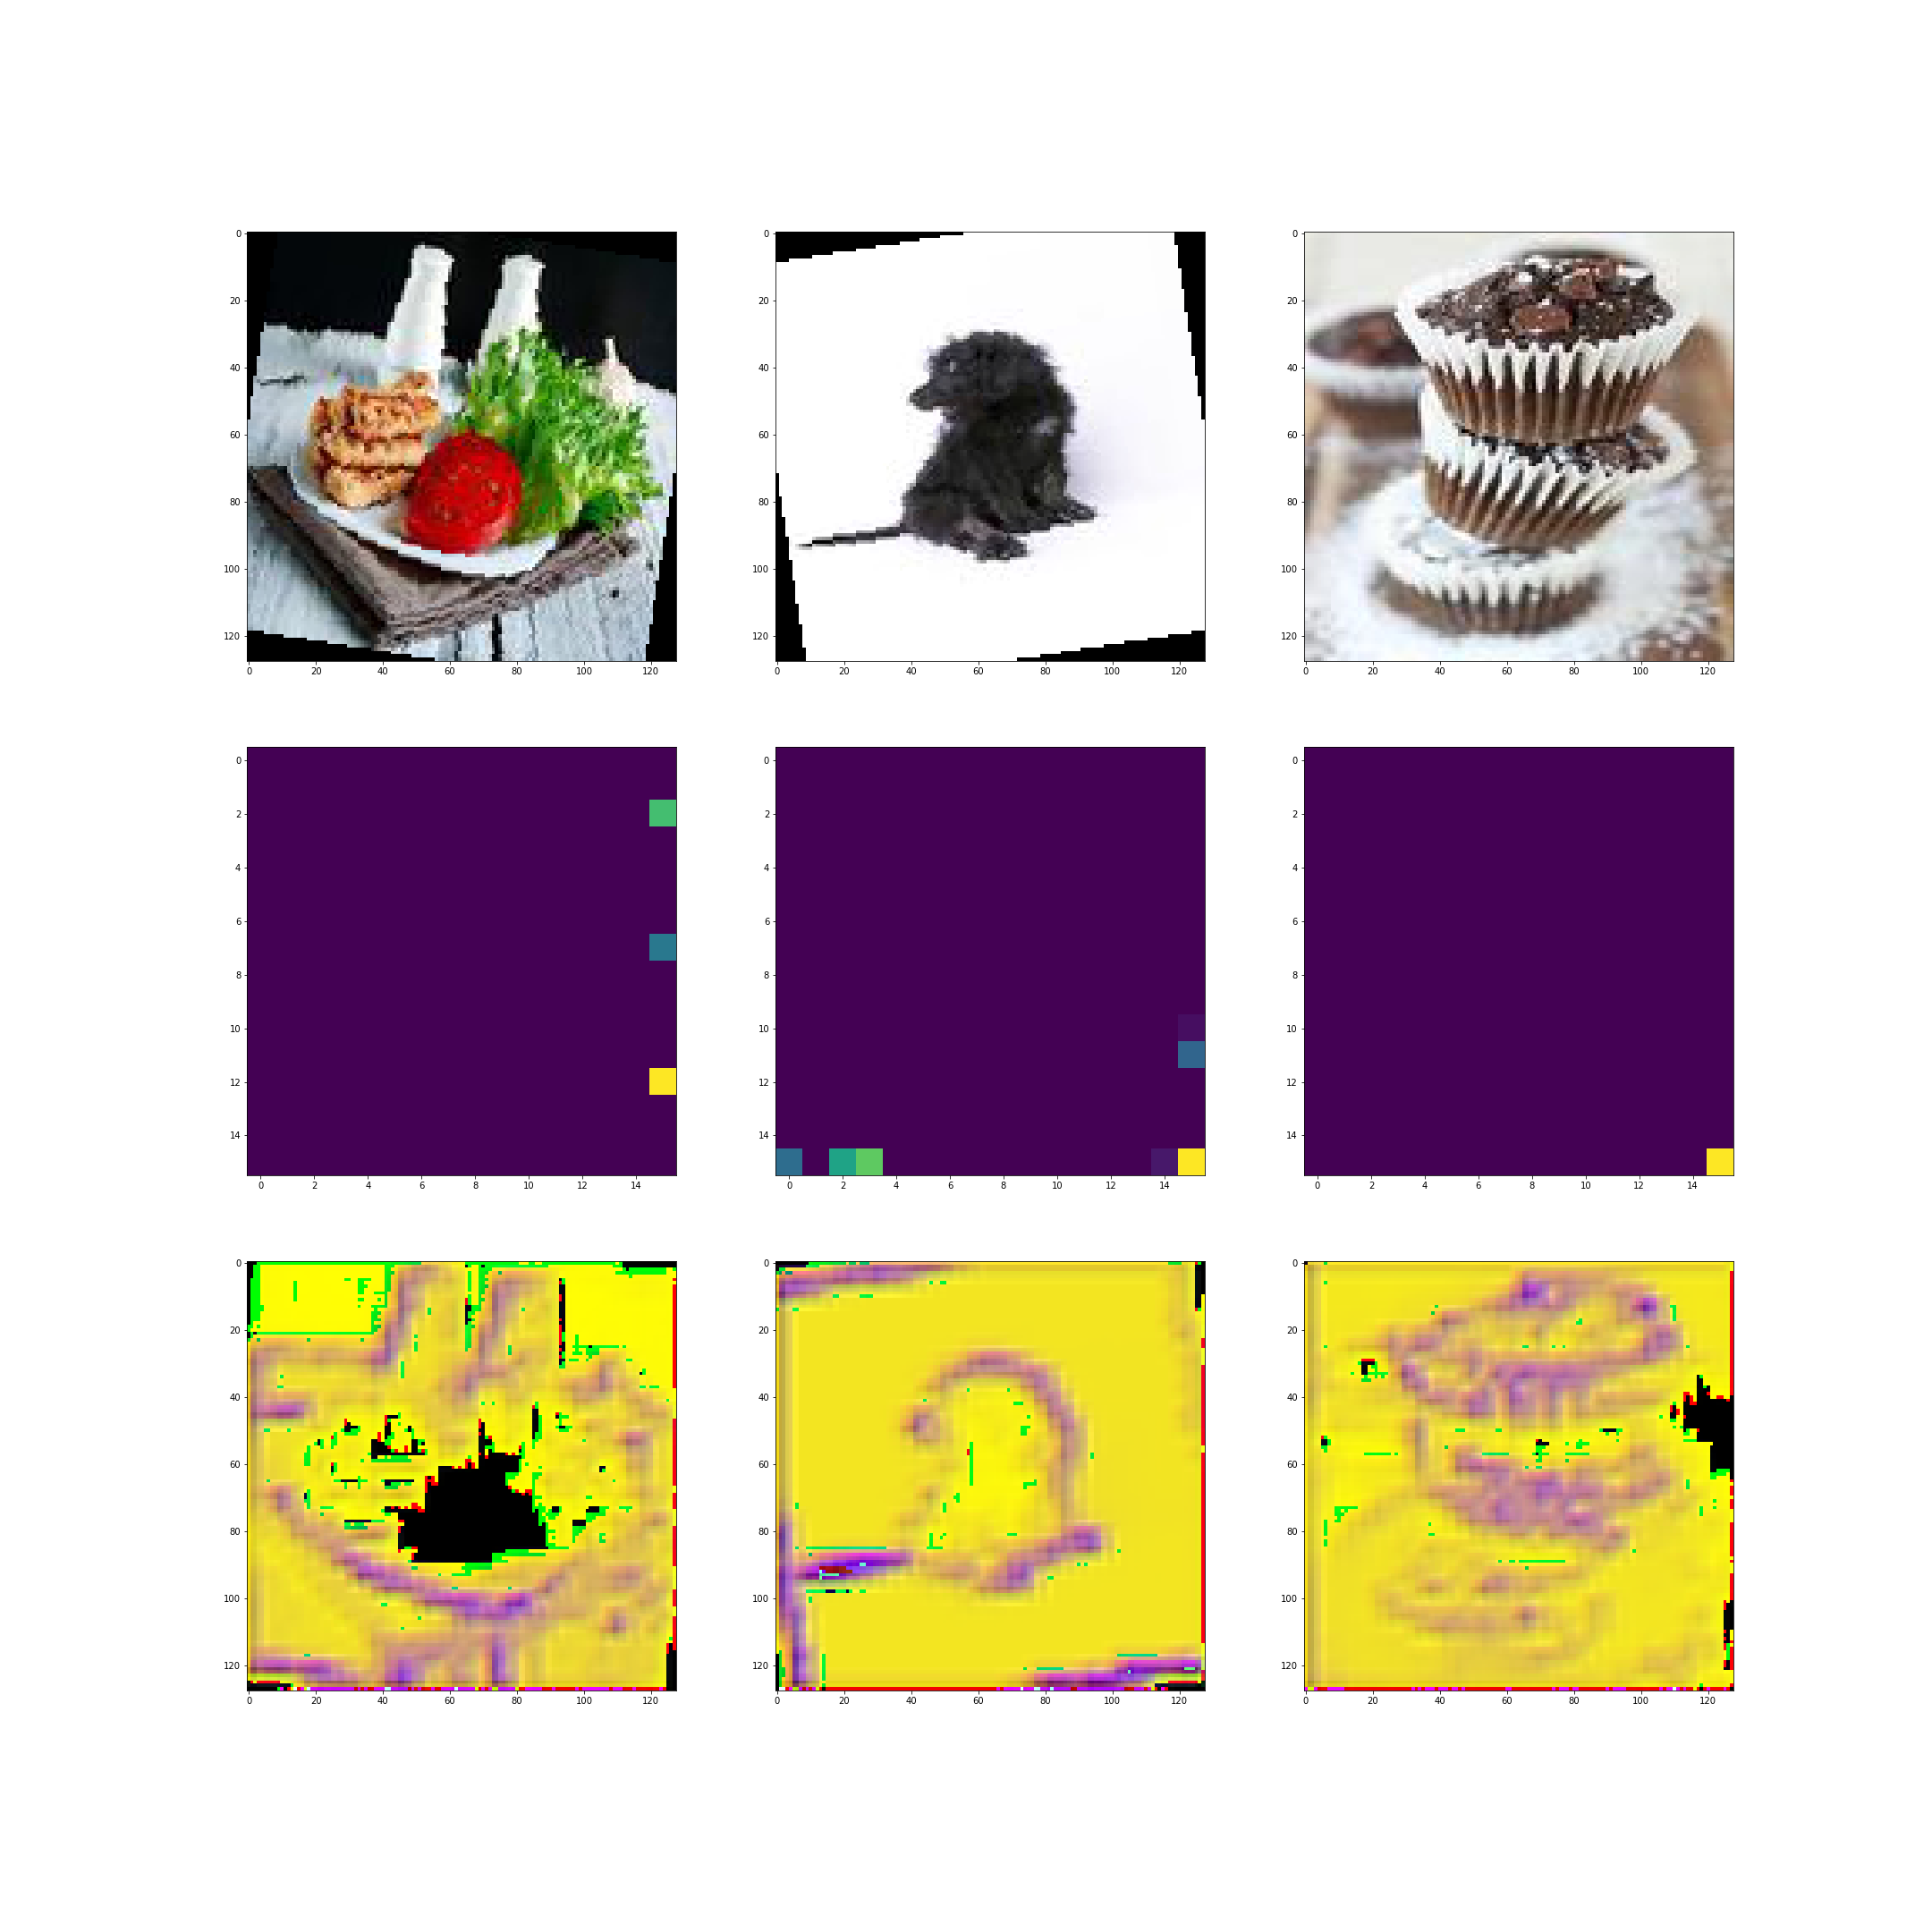
\includegraphics[width=0.7\linewidth]{../diagrams/node8_layer3_DMF}
	\caption{Node 8, Layer 3}
	\label{fig:node8layer3dmf}
\end{figure}
\begin{figure}[H]
	\centering
	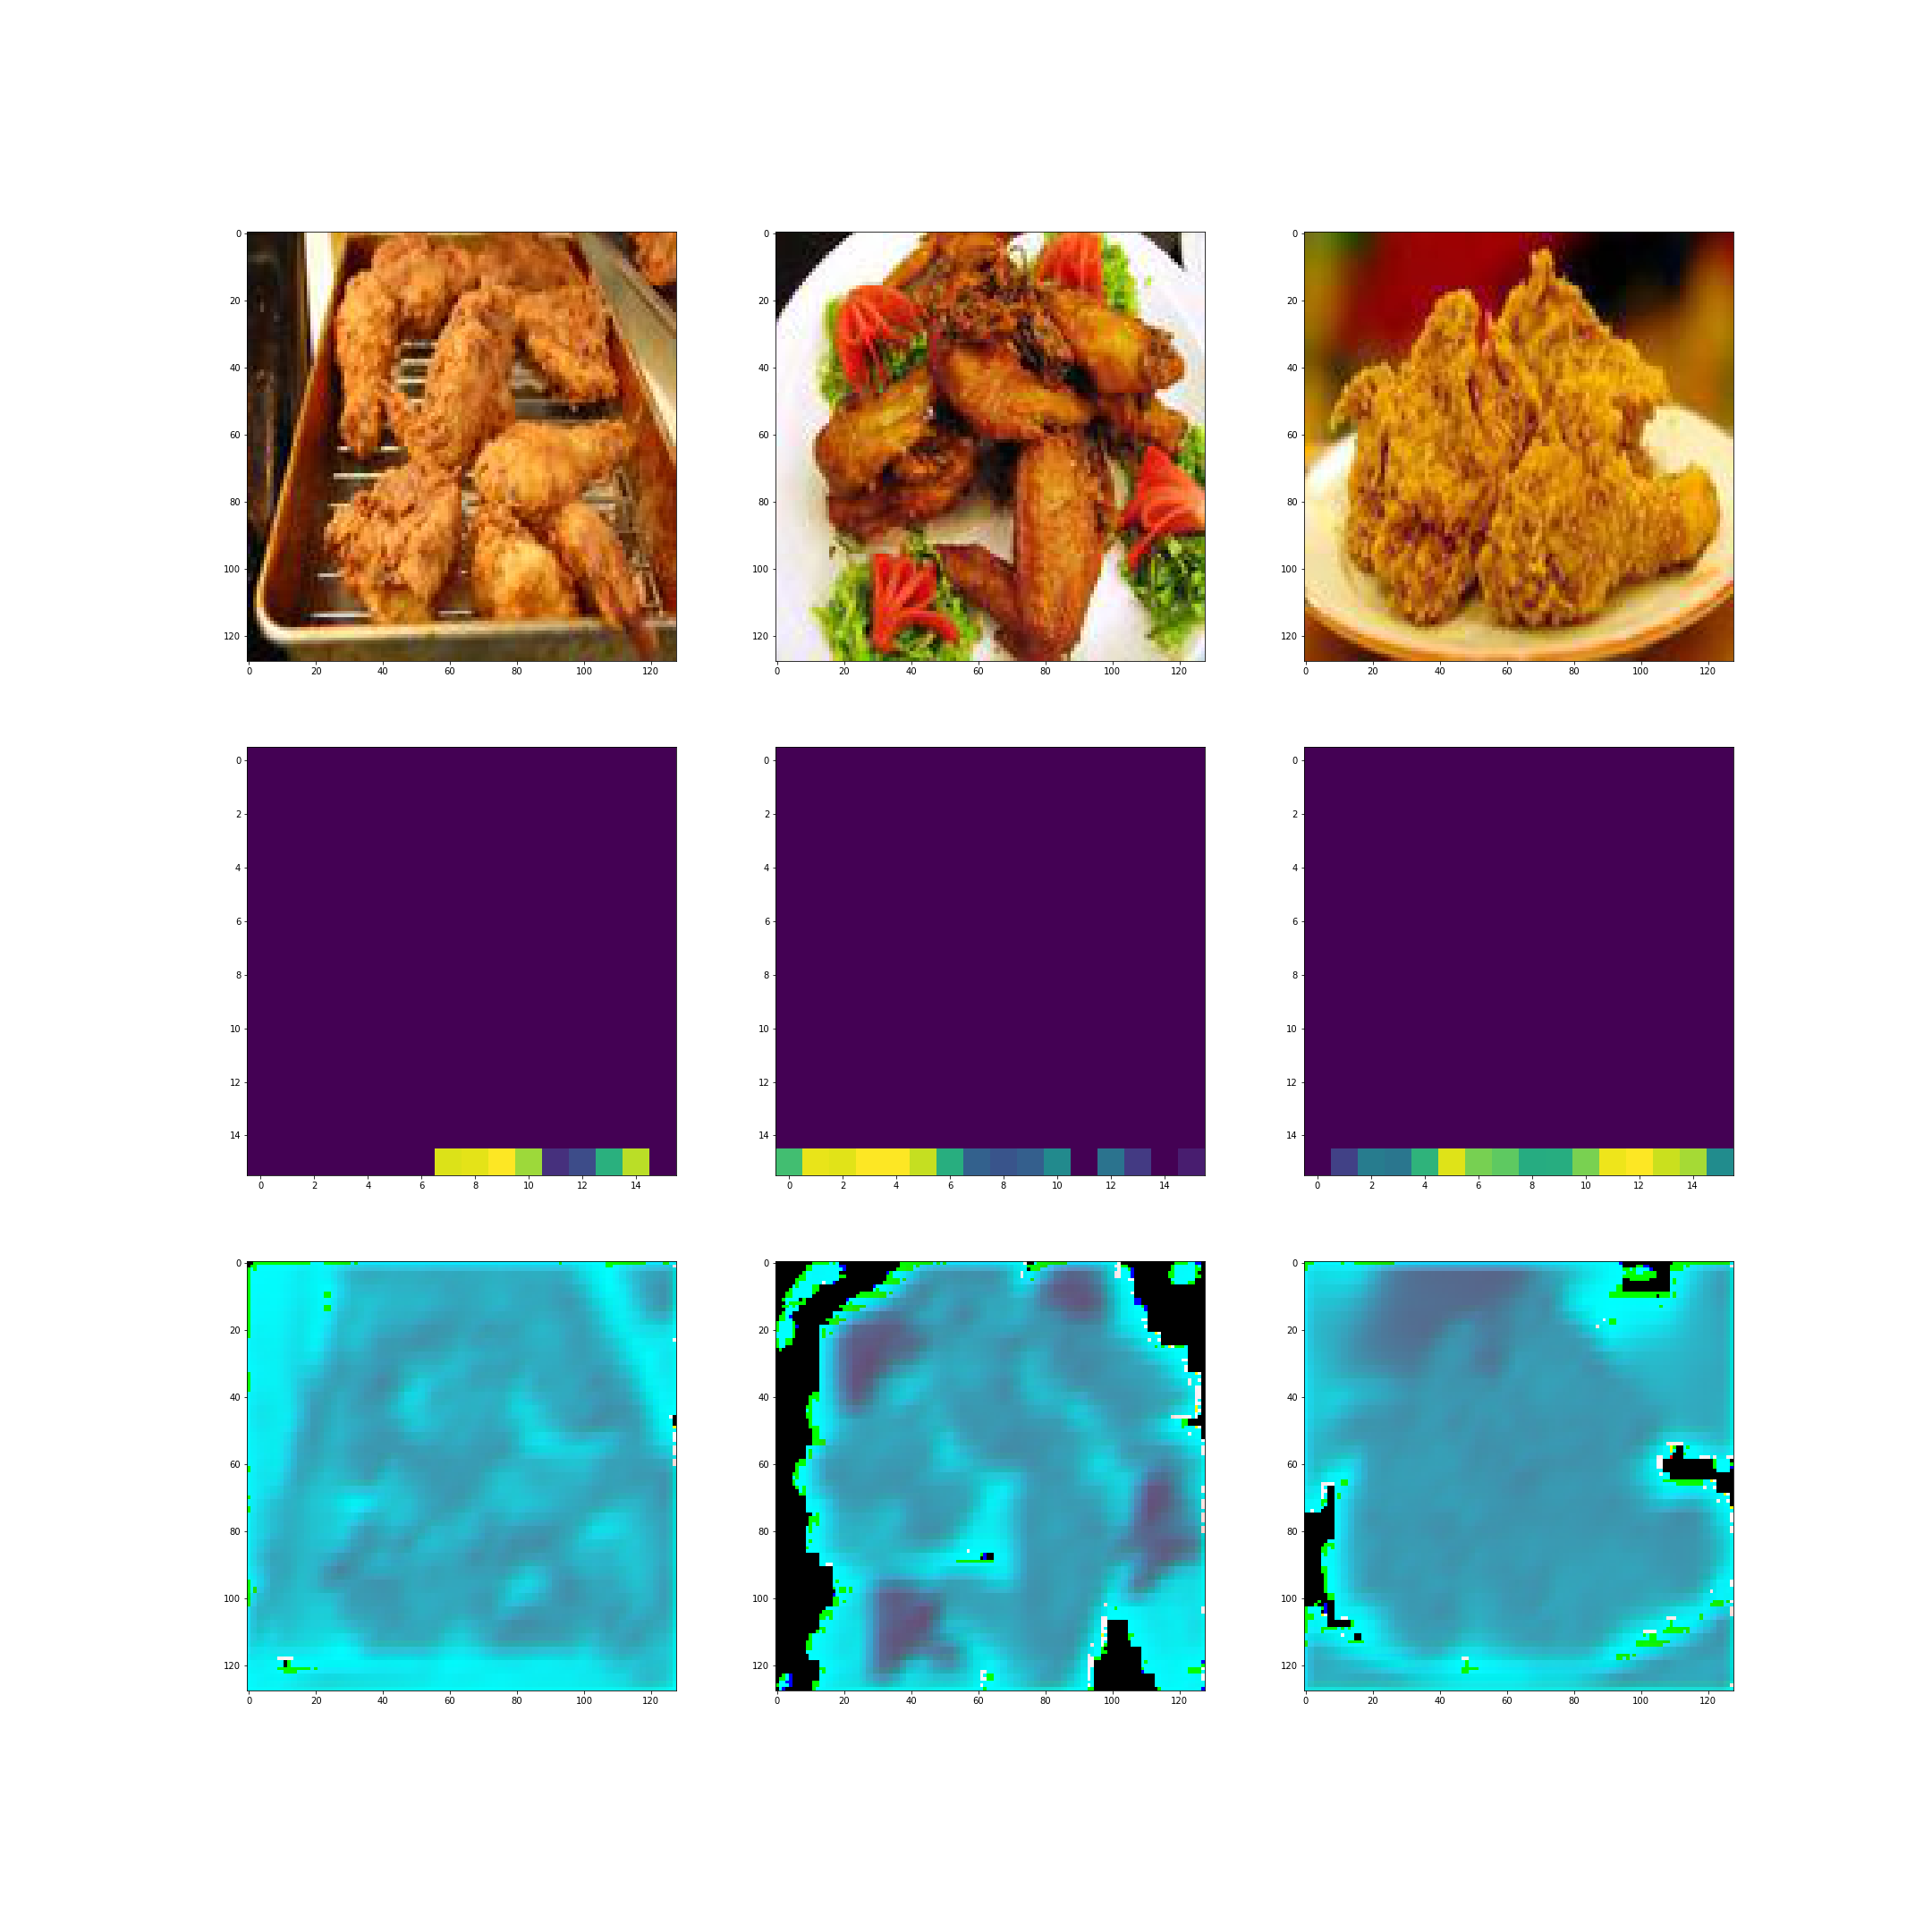
\includegraphics[width=0.7\linewidth]{../diagrams/node15_layer3_DMF}
	\caption{Node 15, Layer 3}
	\label{fig:node15layer3dmf}
\end{figure}
\begin{figure}[H]
	\centering
	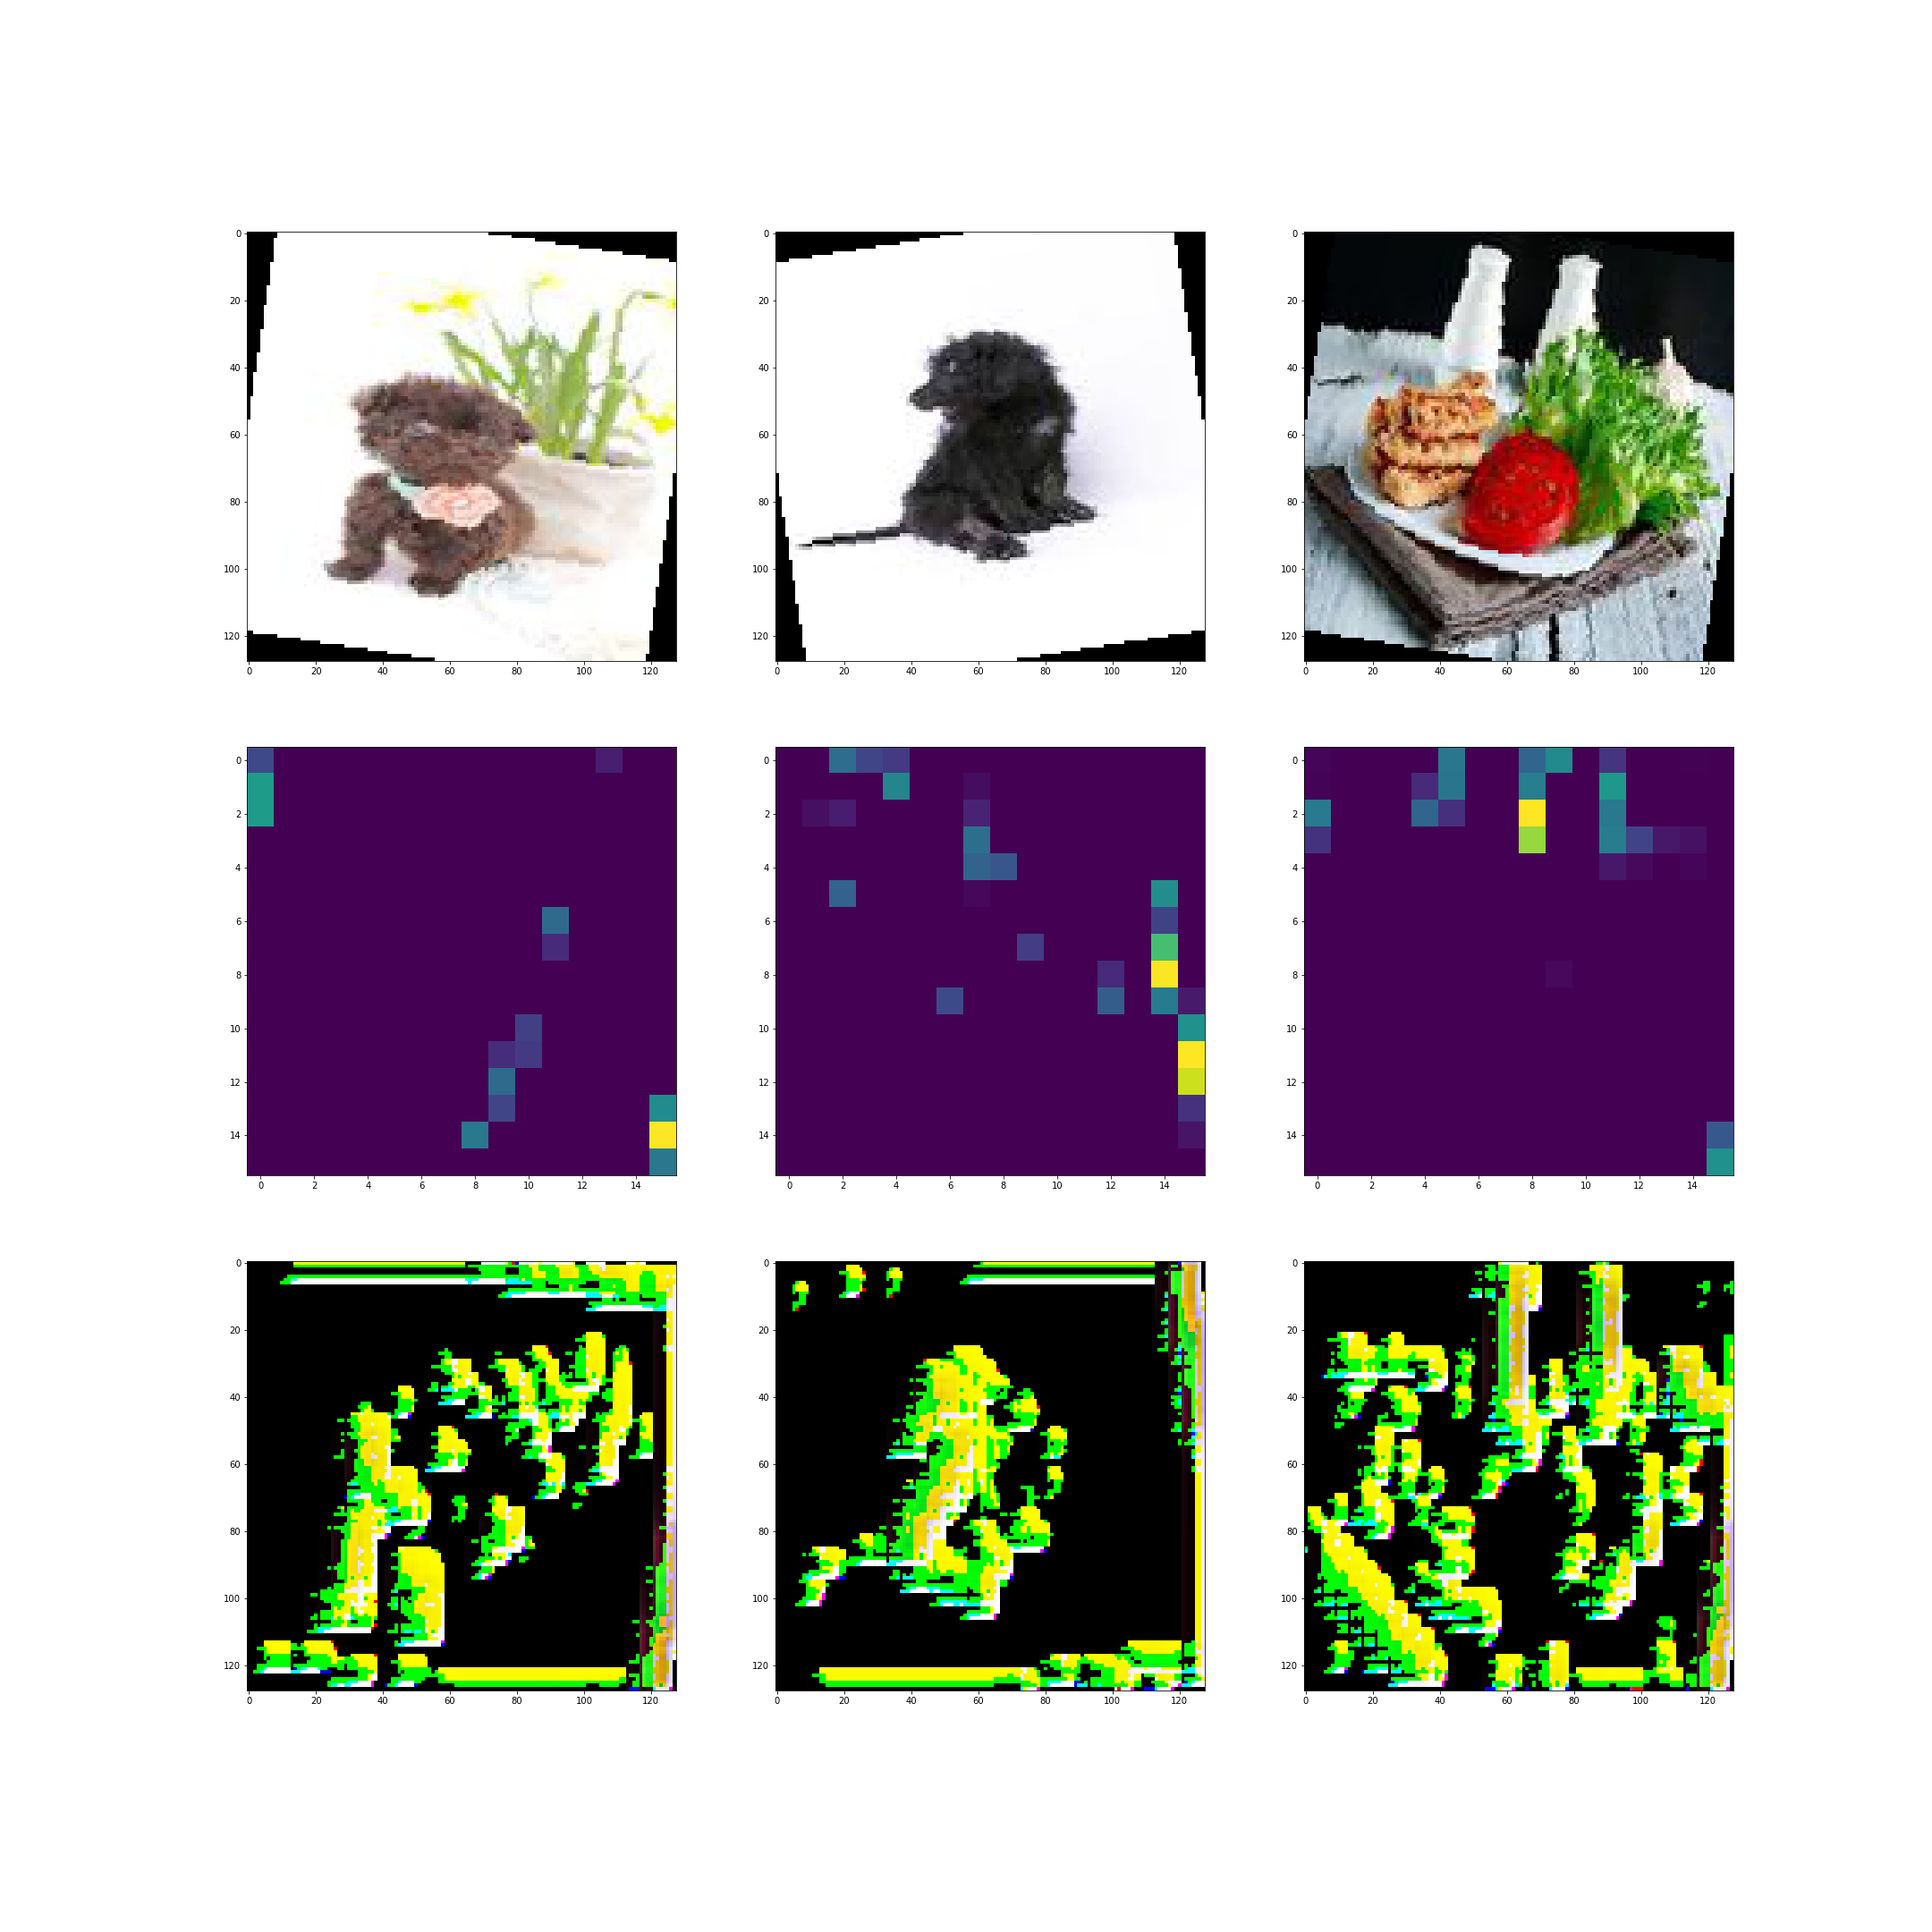
\includegraphics[width=0.7\linewidth]{../diagrams/node23_layer3_DMF}
	\caption{Node 23, Layer 3}
	\label{fig:node23layer3dmf}
\end{figure}

We can see some indications of over-fit as node 15 in layer 2 and 3 (\textit{Figures 21 and 23}) seem to pixels with no identifiable pattern. This presents a possible concrete application of feature visualization as a tool to identify nodes that have been over-fit and potentially estimate reasonable network architectures. \\

Notoriously, node 23 in layer 1 (\textit{Figure 20}) has clearly trained to detect textures (probably for fried chicken). \\

Most interestingly, there is also a clear relationship between the position of the node and its activation preference downstream. Node 8 in the first layer (\textit{Figure 18}), seemed to activate maximally with edges (note the mesh grid and the edge of the rotated muffin picture) and developed further specificity in deeper layers. The can be observed with node 23.  There is no obvious reason for such behavior, since our architecture even has different width between these layers. Potentially, this could suggest that the network develops "pathways" (similar to visual pathways in the brain) that have some coherent organization within the network's architecture. A tantalizing possibility is that deeper neural network architectures exhibit high performances as it allows pathways to develop greater downstream specificity. Instead of trying to use "more" features from our input, it can better identify each. \\

Finally, we look for differences in layer-wide activation for sample images with different labels.

\begin{figure}[H]
\centering
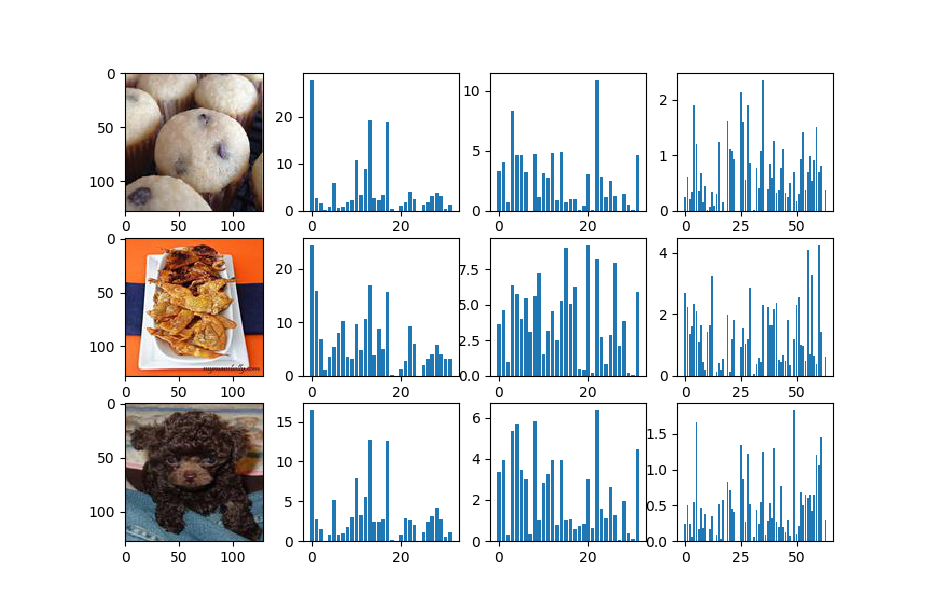
\includegraphics[width=0.7\linewidth]{../diagrams/layeracts3}
\caption{From left to right: layer-wide activation per layer measure as the F-norm}
\label{fig:layeracts3}
\end{figure}
\begin{figure}[H]
\centering
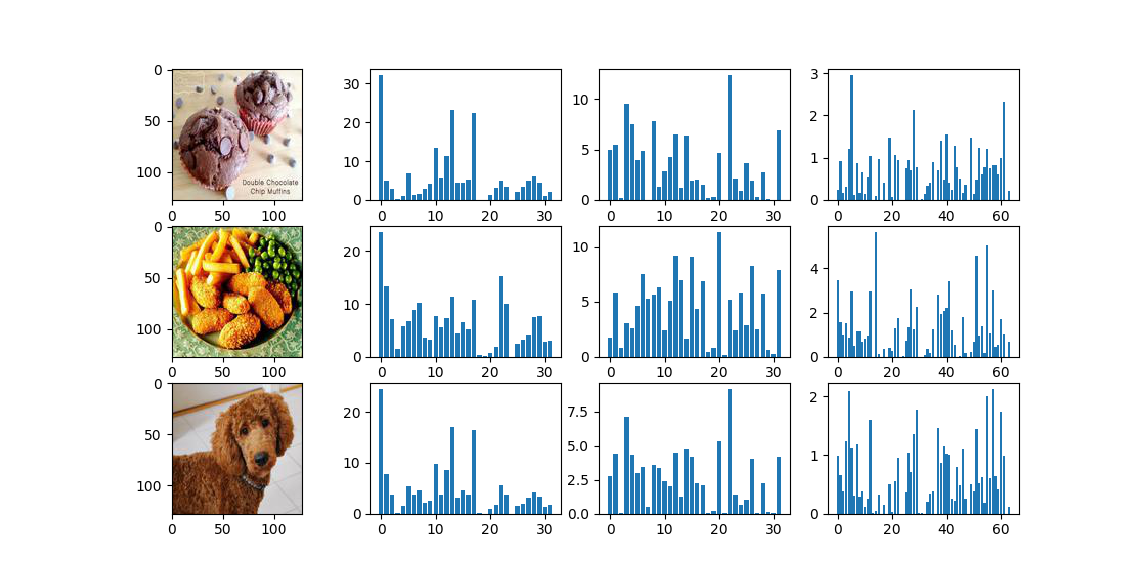
\includegraphics[width=0.7\linewidth]{../diagrams/layeracts1}
\caption{From left to right: layer-wide activation per layer measure as the F-norm}
\label{fig:layeracts1}
\end{figure}


\section{Discussion \& Further Work}

Overall, we have seen that weight visualization works well for early layers that perform one-to-one operations, but lose all interpretability if not. This is particularly true for convolutional neural networks and networks with varying dimensions through its intermediate layers. \\

Feature-map visualization are a fairly easy and intuitive method to visualize intermediate layers of ``reasonable" dimensions (i.e. layers that have dimensions somewhat similar to the input). \\

Deconvnet visualization requires some work in its implementation but is able to deal with multi-channel data and hidden layers in increasingly complex architectural networks. Although we dealt with images that were fairly small (128x128 pixels at most), deconvnet methods can also help identify specific areas of activation within larger images. \\

We only performed rudimentary optimization over our validation-set, but more sophisticated alternatives exist. In particular, (Olah et al., 2017) \cite{distill}, generates images of maximum activation for a specific filter or layer. These are easily implemented in a CAFFE environment, but require more time to apply to tensorflow. The methodology, however, is fairly straightforward in that it takes the gradient over the entire pixel-space initially, or tiled subsets thereof, and ``ascends" towards maximum activation. The images produced are incredibly interesting but of limited interpretability and are computationally expensive. \\

Feature visualization, in all its forms, can serve as a guideposts for architectural design of neural networks. First, we can use it to isolate over-fit nodes by noticing single-pixel activation across different input. More abstractly, if we notice some "obvious" discriminant features are not differentially activating our nodes (obvious is relative to the dataset and classification objective, naturally), this may suggest the need for more parameters. With current development, practitioners can readily visualize their nodes to look for anomalies in their implementation.\\


Many questions, however, remain unanswered. An interesting problem is the variability of feature visualization across training runs. The most obvious challenge of this path of inquiry is that more complex datasets, with more interesting discriminant features, require more resources to train. \\

Similarly, feature visualization can guide the development of statistical tests which can eventually determine nodes that are ``lazy" vs. ``active". Ideally, this would lead to optimization methods that can, with an already trained network, suggest architectural improvements improvements (cf: Lengerich et al. 2017)\cite{resampling}. \\

On the other hand, intuition continues to be an important part of neural network implementation. As such, images can help guide users who do not have the computational resources to retrain large neural networks to determine if "out-of-the-box" classification for untrained data is feasible. This would be a very heuristic process, but one which undeniably remains an important component in the use and development of neural networks. \\

\pagebreak

\bibliographystyle{unsrt}
\bibliography{MLreferences}
\end{document}
